\documentclass[12pt, letterpaper]{article}

%==========

\setlength{\oddsidemargin}{0in}  %left margin position, reference is one inch
\setlength{\textwidth}{6.5in}    %width of text=8.5-1in-1in for margin
\setlength{\topmargin}{-0.5in}    %reference is at 1.5in, -.5in gives a start of about 1in from top
\setlength{\textheight}{9in}     %length of text=11in-1in-1in (top and bot. marg.) 

%==============Packages & Commands=================

%========== MS
\usepackage{soul}
\usepackage{amsmath,amssymb}
\usepackage{graphicx}% Include figure files
\usepackage{caption}
\usepackage{color}% Include colors for document elements
\usepackage{dcolumn}% Align table columns on decimal point
\usepackage{bm}% bold math

\usepackage[natbibapa]{apacite}
\bibliographystyle{apacite}

%\usepackage{todonotes}

\usepackage{fontspec}
\usepackage{polyglossia}

\usepackage{setspace}

\usepackage{enumitem}

\usepackage{changepage}

\usepackage{lipsum}

\usepackage{scrextend}

\usepackage{booktabs}

\usepackage{subfigure}

\usepackage{longtable}
\usepackage{ltxtable} 
\usepackage{tabularx}
\usepackage{changepage}
\usepackage{float}
%\usepackage{fancyhdr}

%===============Some new commands==================
\newcommand{\myparagraph}[1]{\paragraph{#1}\mbox{}\\}

\usepackage{titling}

\newcommand{\subtitle}[1]{%
	\posttitle{%
		\par\end{center}
	\begin{center}\large#1\end{center}
	\vskip0.5em}%
}

\newcommand*\samethanks[1][\value{footnote}]{\footnotemark[#1]}

\newcommand{\bscom}[2]{%
	% #1 Original text.
	% #2 Replacement text.
	\st{#1}{\color{blue}\fontsize{8}{8}\selectfont\,#2}}


\RequirePackage{color}
\RequirePackage{soul}
\setstcolor{blue}

\newcommand{\com}[1]{%
	% #1 Original text.
	% #2 Replacement text.
	{\color{blue}\fontsize{8}{8}\selectfont\,#1}}
    
 \newcommand{\red}[1]{%
	% #1 Original text.
	% #2 Replacement text.
	{\color{red}\fontsize{14}{14}\selectfont\,#1}}

 \newcommand{\ms}[1]{%
	% #1 Original text.
	% #2 Replacement text.
	{\color{green}\fontsize{14}{14}\selectfont\,#1}}



%============Article Title, Authors================




\title{Veränderung der Kommunikation im Bundestag seit dem Einzug der AfD 2017}
\subtitle{Kommunikationstheoretische Analyse der Bundestagsprotokolle}

\author{Nils Heinemann \thanks{Politics, Administration \& International Relations}  \\[3ex] Vivian Clausen \thanks{Comunication, Culture \& Management} \and Mehmet Cetin \thanks{Sociology, Politics \& Economics} \\[3ex] Joseph Oertel \thanks{Politics, Administration \& International Realtions}\\[3ex]}
%\date{}


\begin{document}
	
	\maketitle
	\doublespacing
	

\centerline{\textbf{Zeppelin Projekt}}
\centerline{\textbf{Betreuer: Michael Scharkow}}
\vspace{1cm}


\begin{abstract}

\begin{singlespace}
 \textit{\lipsum[3]}
\end{singlespace}



\end{abstract}
	
	\clearpage
	
	%================Begin Manuscript==================
	\newpage
	\tableofcontents
	\section{General Thoughts/Ideas}

\begin{itemize} 
\item [] {\bfseries Hypothese 1:} 
Die Themen der Parlamentsdebatten haben sich geändert
\item  Hypothese 1a: Die Themen sind einseitiger geworden und es wird insgesamt über weniger Themen diskutiert
\item  Hypothese 1b: Es wird öfter am inhaltlich am Tagesordnungspunkt vorbei diskutiert 
\item [] {\bfseries Hypothese 2:} 
Die Sprachverständlichkeit der Politiker nimmt ab
\item [] {\bfseries Hypothese 3:} 
Die AfD ist die isolierteste Partei und andere Parteien isolieren sich auch zunehmends 
\item [] {\bfseries Hypothese 4:} 
Kommunikation hat sich auf sprachlicher Ebene verändert und ist
\item[] 4a: Streitkultur hat sich durch mehr Kritik und Widerspruch auf persönlicher Ebene verschärft
\item[] 4b: Sprachlicher Ausdruck des gegenseitigen Respekts hat abgenommen 

\end{itemize}






\newpage
	\section{Introduction}

	\section{Literature}


\newpage	
	\section{Theory \& Hypotheses}




\newpage
	\section{Methodology and Data}
\subsection{Methodologie der Arbeit}
Als Daten wurden die Bundestagsprotokolle im Zeitraum von 2009 bis 2018 von der Bundestagswebsite\thanks {https://www.bundestag.de/service/opendatav}  heruntergeladen und in einen R Datensatz eingelesen. Die Daten der Bundestagsprotokolle vor 2017 mussten mit Hilfe von regulären Ausdrücken in den Datensatz eingelesen werden, da der Inhalt der Protokolle nicht mit XML-Nodes aufgegliedert ist. Dafür wurde auch die Stammdatendatei der Politiker im Bundestag verwendet, um die Namen der Politiker als Redner in den entsprechenden Legislaturperioden identifizieren zu können. Die folgende Funktion beispielsweise teilt den Text in Reden ein, indem Sie nach dem Muster sucht, dass dem einer Rede entspricht. Dieses Muster ist für alle Protokolle gegeben durch den Namen von einem Politiker gefolgt von seiner Partei in Klammern und einem Doppelpunkt, oder der Name von einem Politiker gefolgt von einem Doppelpunkt, wenn dieser keiner Partei angehört.
\begin{verbatim}
str_split(text, paste0(c("(?<=.)(?=(",namenregex,")(?=(:| (\\(.{1,40}\\):))))")
,collapse = ""))
\end{verbatim}
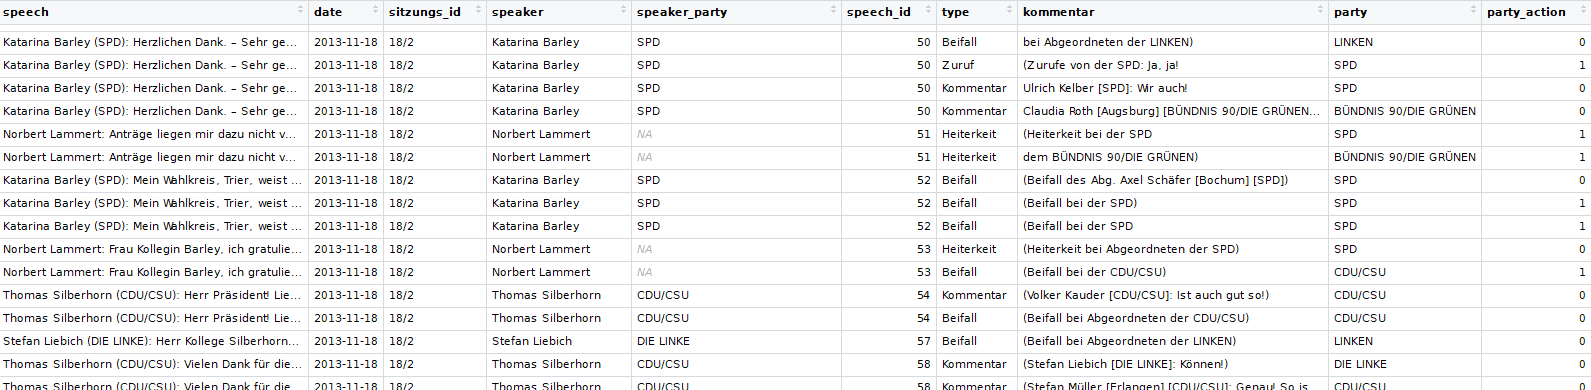
\includegraphics[width=\linewidth]{Grafiken/Head_Reden.PNG}
\\

\subsection{Methodologie der Hypothesen}
{\bfseries Hypothese 1:} Zur Überprüfung dieser Hypothese wurde eine Stichprobe aus den Plenarprotokollen gezogen, die anschließend von Hand kodiert wurde. Für eine Vergleichbarkeit der Ergebnisse besteht die Stichprobe aus jeweils 60 Reden, die in dem ersten Jahr nach Beginn der Legislaturperiode abgehalten wurden. Die Stichprobe wurde in zwei Schritten erstellt: Aus jedem Zeitraum wurden 59 Plenarprotokolle ausgewählt, das sind 2017 alle Protokolle, 2013 eine Auswahl aus 60 und 2009 eine Auswahl aus 67 Protokollen. Aus jeder der 60 Plenarprotokollen wurde eine Rede zufällig ausgewählt und den Kodierern zufällig zugeteilt. Zusätzlich wurden 10 Reden pro Kodierer auf zwei weitere Kodierer aufgeteilt, die einem späteren Reliabilitätstest dienen. Ein Beispiel für die Stichprobe:  \\
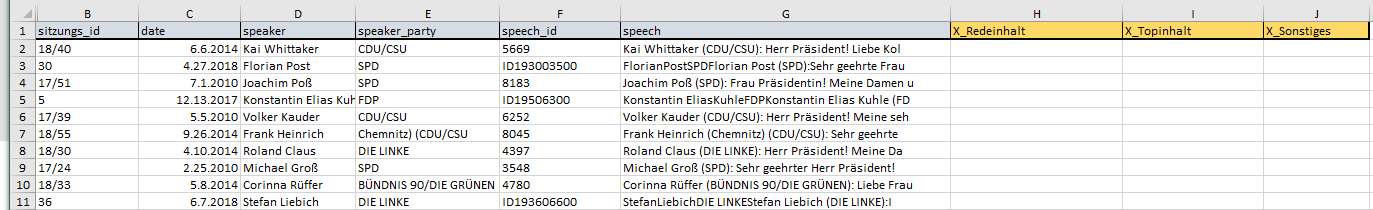
\includegraphics[width=\linewidth]{Grafiken/Head_Stichprobe.PNG}\\

{\bfseries Hypothese 2:} Zur Überprüfung der Sprachverständlichkeit wurden alle \verb 48.919  Reden im Zeitraum von 2009 bis 2017 analysiert. Für jeden Monat wurden alle Reden jeder einzelnen Partei pro Monat gruppiert und anschließend, in Silben, Wörter und Sätze aufgegliedert. Aus diesen Daten wurde der FLESCH-Index berechnet, einer der etabliertesten Readability-Indizes in der Sprachverständlichkeitsforschung. \\
{\bfseries Hypothese 3:} Zur Überprüfung der Hypothese, welche Partei wie isoliert ist, wurden alle \verb 445.301  Interaktionen im Bundestag im Zeitraum von 2009-2017 analysiert. Zusätzlich wurden die häufigsten verwendeten Wörter der Parteien analysiert. \\
{\bfseries Hypothese 4:} 
Kombination aus qualitativer Untersuchung von Kommentaren in ihren jeweiligen Reden-Kontext und die quantitative Untersuchung von stilistischen Merkmalen sprachlicher Veränderung. 


\newpage
	\section{Results}
\subsection{Hypothese 3}

Aus den Auswertungen der Plenarprotokolle sind folgende Ergebnisse entstanden:
\begin{center}
% latex table generated in R 3.5.0 by xtable 1.8-3 package
% Sun Nov 18 13:22:12 2018
\begin{table}[ht]
	\centering
	\begin{tabular}{lrrrrrrrl}
		\hline
		Partei & Beifall & Heiterkeit & Kommentar & Lachen & Widerspruch & Zuruf & Summe & Periode \\ 
		\hline
		\hline
		SPD & 12311 & 318 & 3346 & 231 & 109 & 373 & 16315 & 17-18 \\ 
		CDU/CSU & 11659 & 333 & 3847 & 112 &  53 & 223 & 16004 & 17-18 \\ 
		DIE LINKE & 9462 & 125 & 2927 & 142 & 107 & 367 & 12763 & 17-18 \\ 
		GRÜNE & 7417 & 131 & 4205 &  95 &  69 & 335 & 11917 & 17-18 \\ 
		FDP & 8470 & 258 & 2782 &  86 &  36 & 249 & 11632 & 17-18 \\ 
		AfD & 7074 & 129 & 3557 & 291 & 114 & 734 & 11165 & 17-18 \\ 
		\hline
		CDU/CSU & 32638 & 856 & 10018 & 234 & 150 & 1047 & 43812 & 13-17 \\ 
		SPD & 32217 & 934 & 6087 & 124 & 159 & 615 & 39407 & 13-17 \\ 
		GRÜNE & 14148 & 158 & 15363 & 116 & 131 & 791 & 29800 & 13-17 \\ 
		DIE LINKE & 20789 & 282 & 8218 & 153 & 210 & 1221 & 29451 & 13-17 \\ 
		\hline
		SPD & 27330 & 731 & 24078 & 863 & 496 & 2264 & 53064 & 09-13 \\ 
		CDU/CSU & 34131 & 633 & 13515 & 326 & 272 & 1584 & 48719 & 09-13 \\ 
		FDP & 32808 & 577 & 10484 & 333 & 280 & 1499 & 44323 & 09-13 \\ 
		DIE LINKE & 19275 & 308 & 7583 & 299 & 268 & 1199 & 27503 & 09-13 \\ 
		GRÜNE & 11716 & 199 & 13391 & 213 & 178 & 634 & 25537 & 09-13 \\ 
		\hline
	\end{tabular}
\end{table}
\end{center}

\subsubsection{Klatschen für andere Fraktionen}

 Beifall ist eine sehr deutliche Form der Zustimmung, die einfach zu erkennen und leicht interpretierbar ist. Klatscht eine Partei für eine andere, so lässt sich daraus schließen, dass die Partei der Rede zustimmen. Aus den Bundestagsprotokollen geht dabei hervor, welche Partei wann klatscht und ob die ganze Partei in den Beifall einstimmt, oder nur einzelne Abgeordnete. Unsere Analyse hat aus den Protokolle der vergangenen zwei Perioden ausgewertet, welche Partei für welche klatscht und damit Zustimmung signalisiert.   \\

\includegraphics[width=\linewidth]{Grafiken/13_17WerfürWen.png}\\
\includegraphics[width=\linewidth]{Grafiken/13_17WerfürWen_prozent.png}\\
Es zeigt sich, dass die Koalitionsparteien am über alle drei Legislaturperioden hinweg am meisten für einander applaudieren. Sowohl 2009-2013 die FDP, die sehr oft für die CDU/CSU klatscht, als auch die SPD und die CDU/CSU, die 2013-2018 oft für einander applaudieren. \\
....
\subsubsection{Klatschen für die eigene Fraktion}
 \noindent Je häufiger eine Partei für sich selbst klatscht im Verhältnis zum Klatschen für andere Parteien, desto eher ist sie in einer isolierten Position. Sie stimmt nur den eigenen Inhalten zu und hat kaum eine inhaltliche Position mit einer anderen Partei gemeinsam. Eine Analyse über den "Eigenklatschanteil" kann also Aufschluss darüber geben, wie Isoliert eine Partei ist. \\

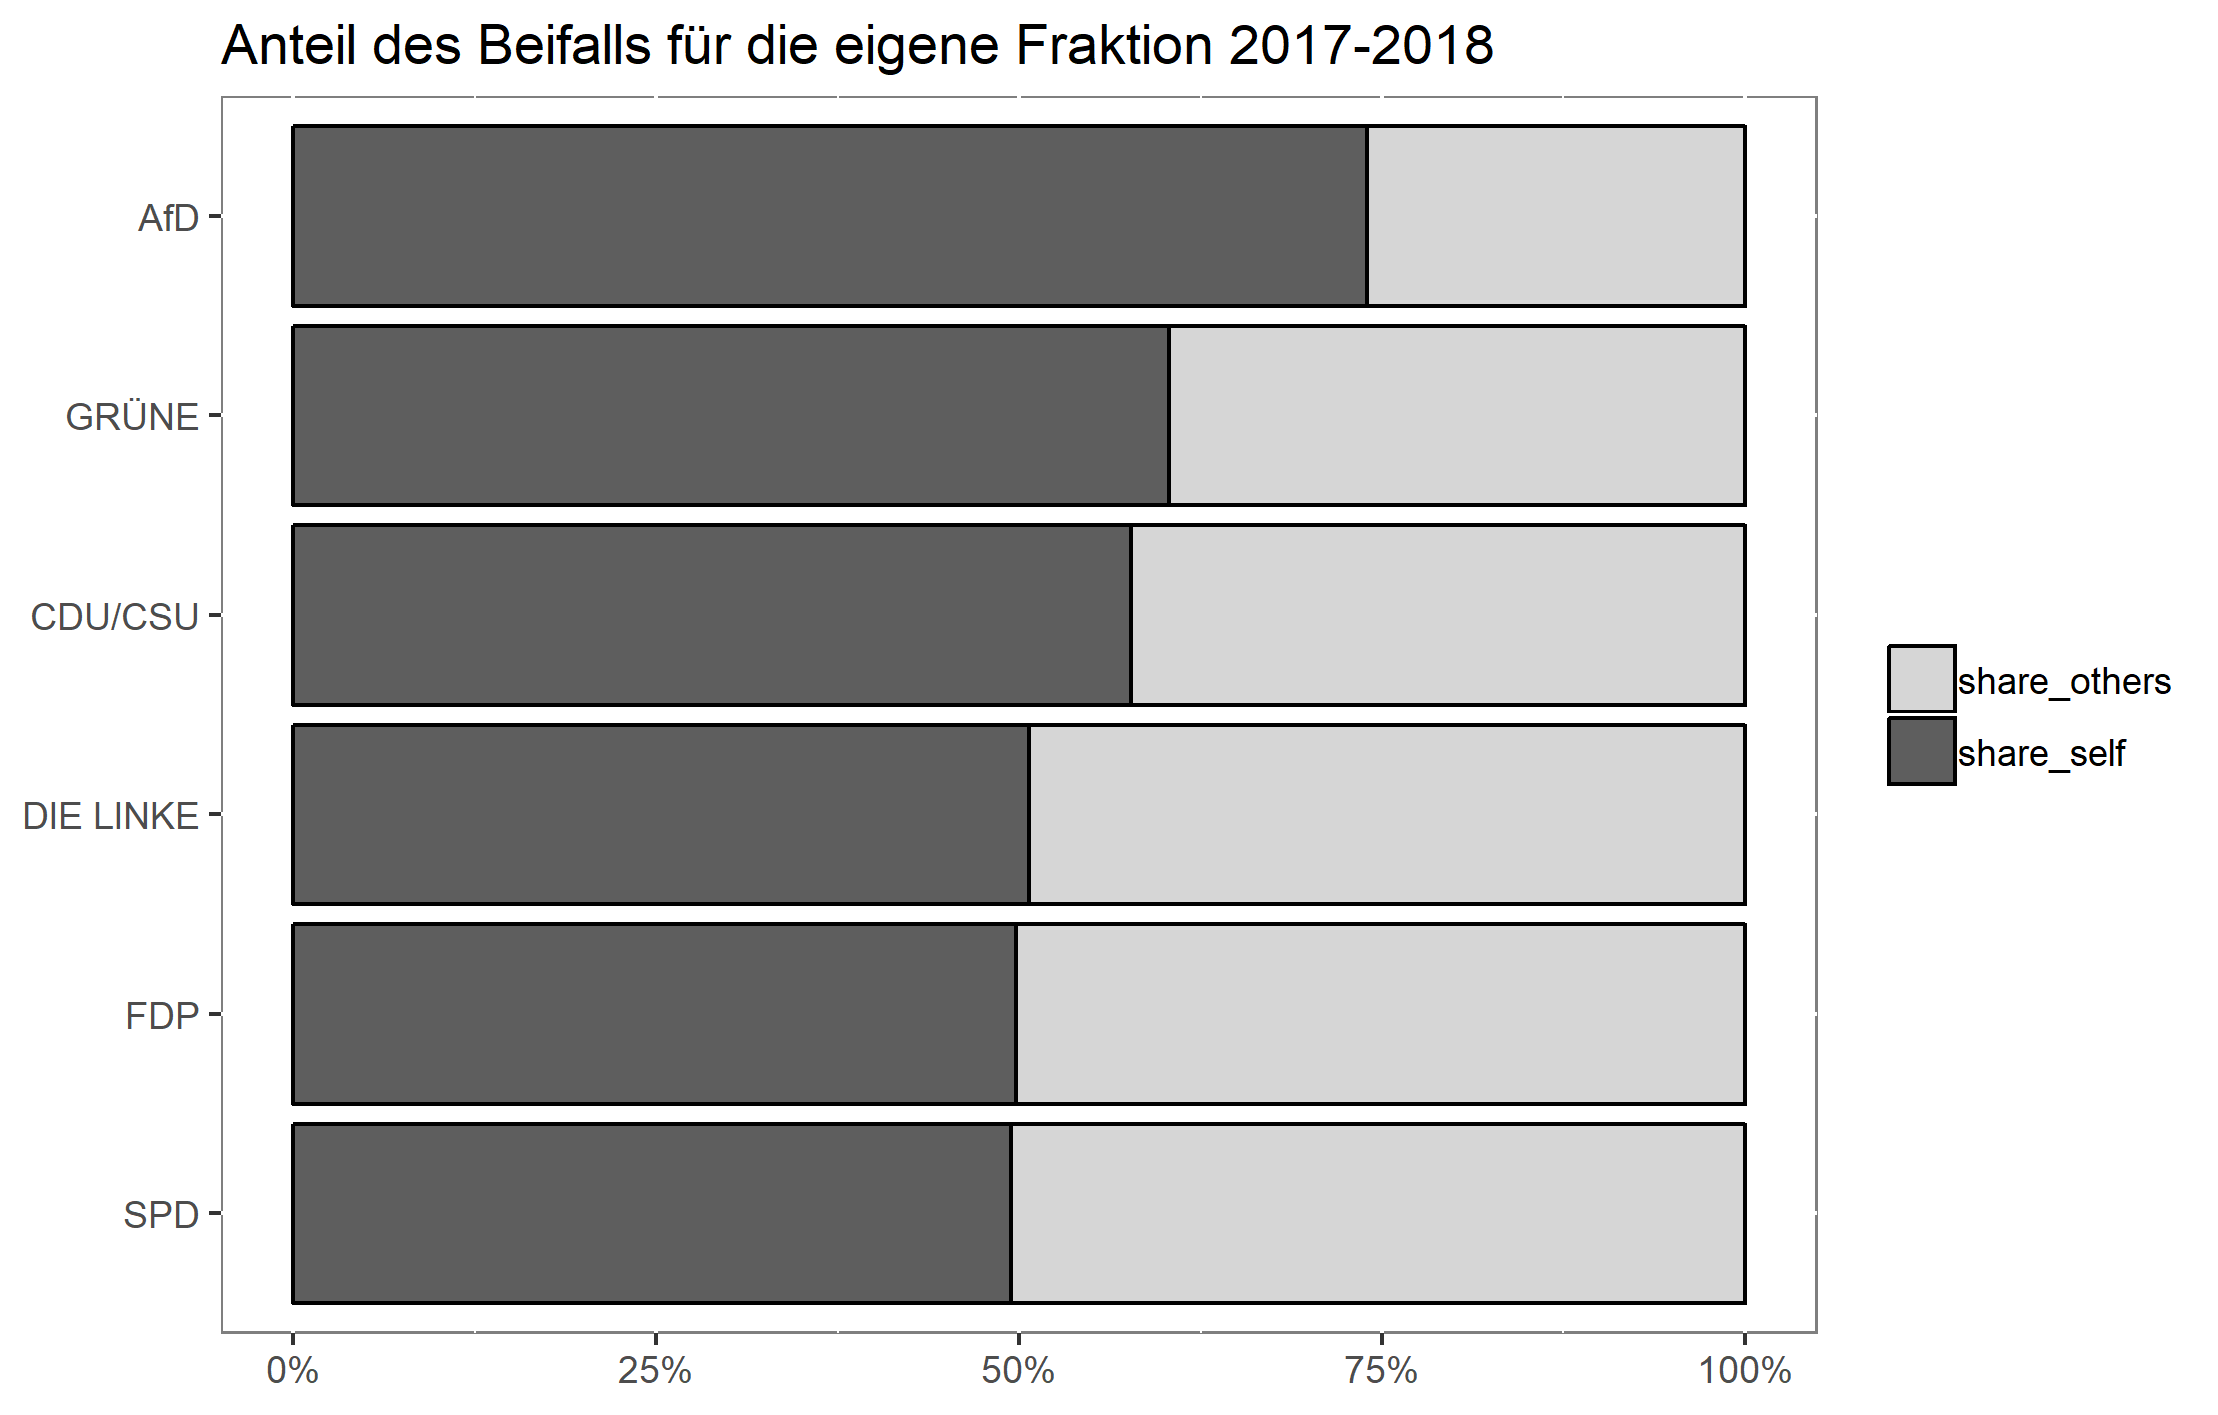
\includegraphics[width=\linewidth]{Grafiken/17_eigenklatschanteil.png}

Die AfD ist demnach die isolierteste Partei. Betrachtet man den "Eigenklatschanteil" im Zeitverlauf zeigt sich, dass auch andere Parteien sich in der momentanen Legislaturperiode zunehmend zu isolieren scheinen. Dass die Kurve am Ende, also gegen Oktober, wieder abfällt, könnte darauf zurückzuführen sein, dass im Monat Oktober zu Beginn unserer Analyse, noch nicht alle Bundestagsreden veröffentlicht waren und daher im Oktober Messzeitpunkte fehlen. \\
  
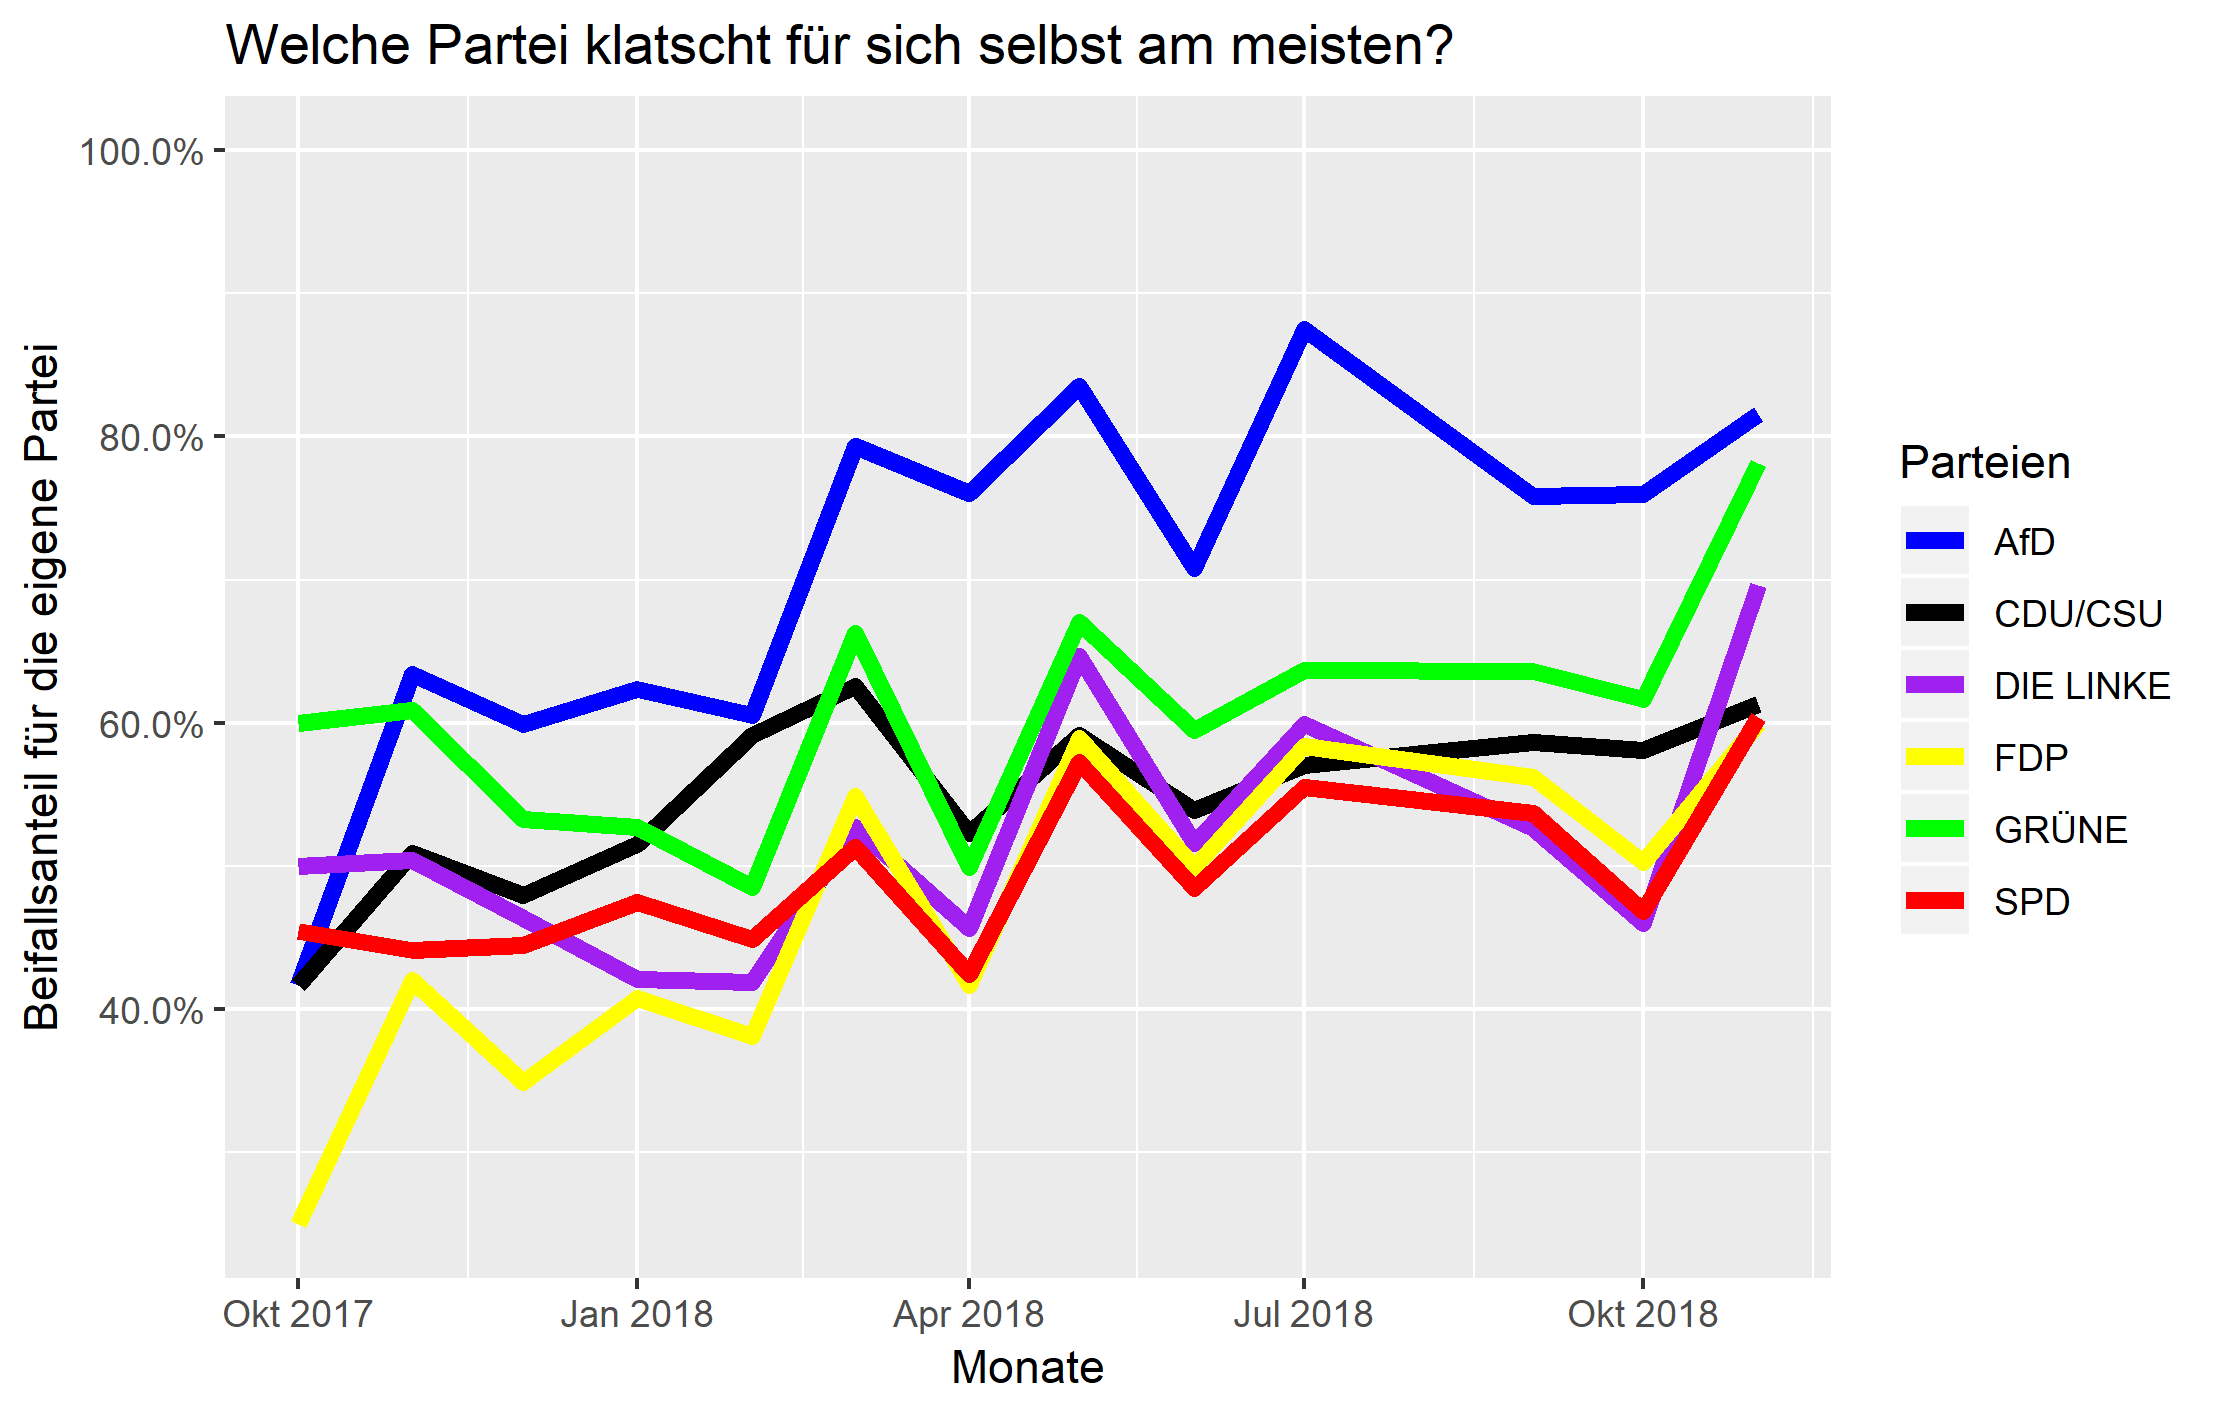
\includegraphics[width=\linewidth]{Grafiken/13_17Zeitverlauf_Klatschen.png}\\

\subsubsection{Geschlossenheit der Parteien}
Ein geschlossenes Auftreten von Parteien nur anhand von gemeinsamen Interaktionen fest zu machen, ist nur begrenzt aussagekräftig. Dennoch sind neben einem kohärenten Inhalt gemeinsame Aktionen ein deutliches Zeichen nach außen, ob eine Partei geschlossen auftritt, oder nicht. Gemeinsamer Beifall ist demnach ein Indikator für Geschlossenheit. \\

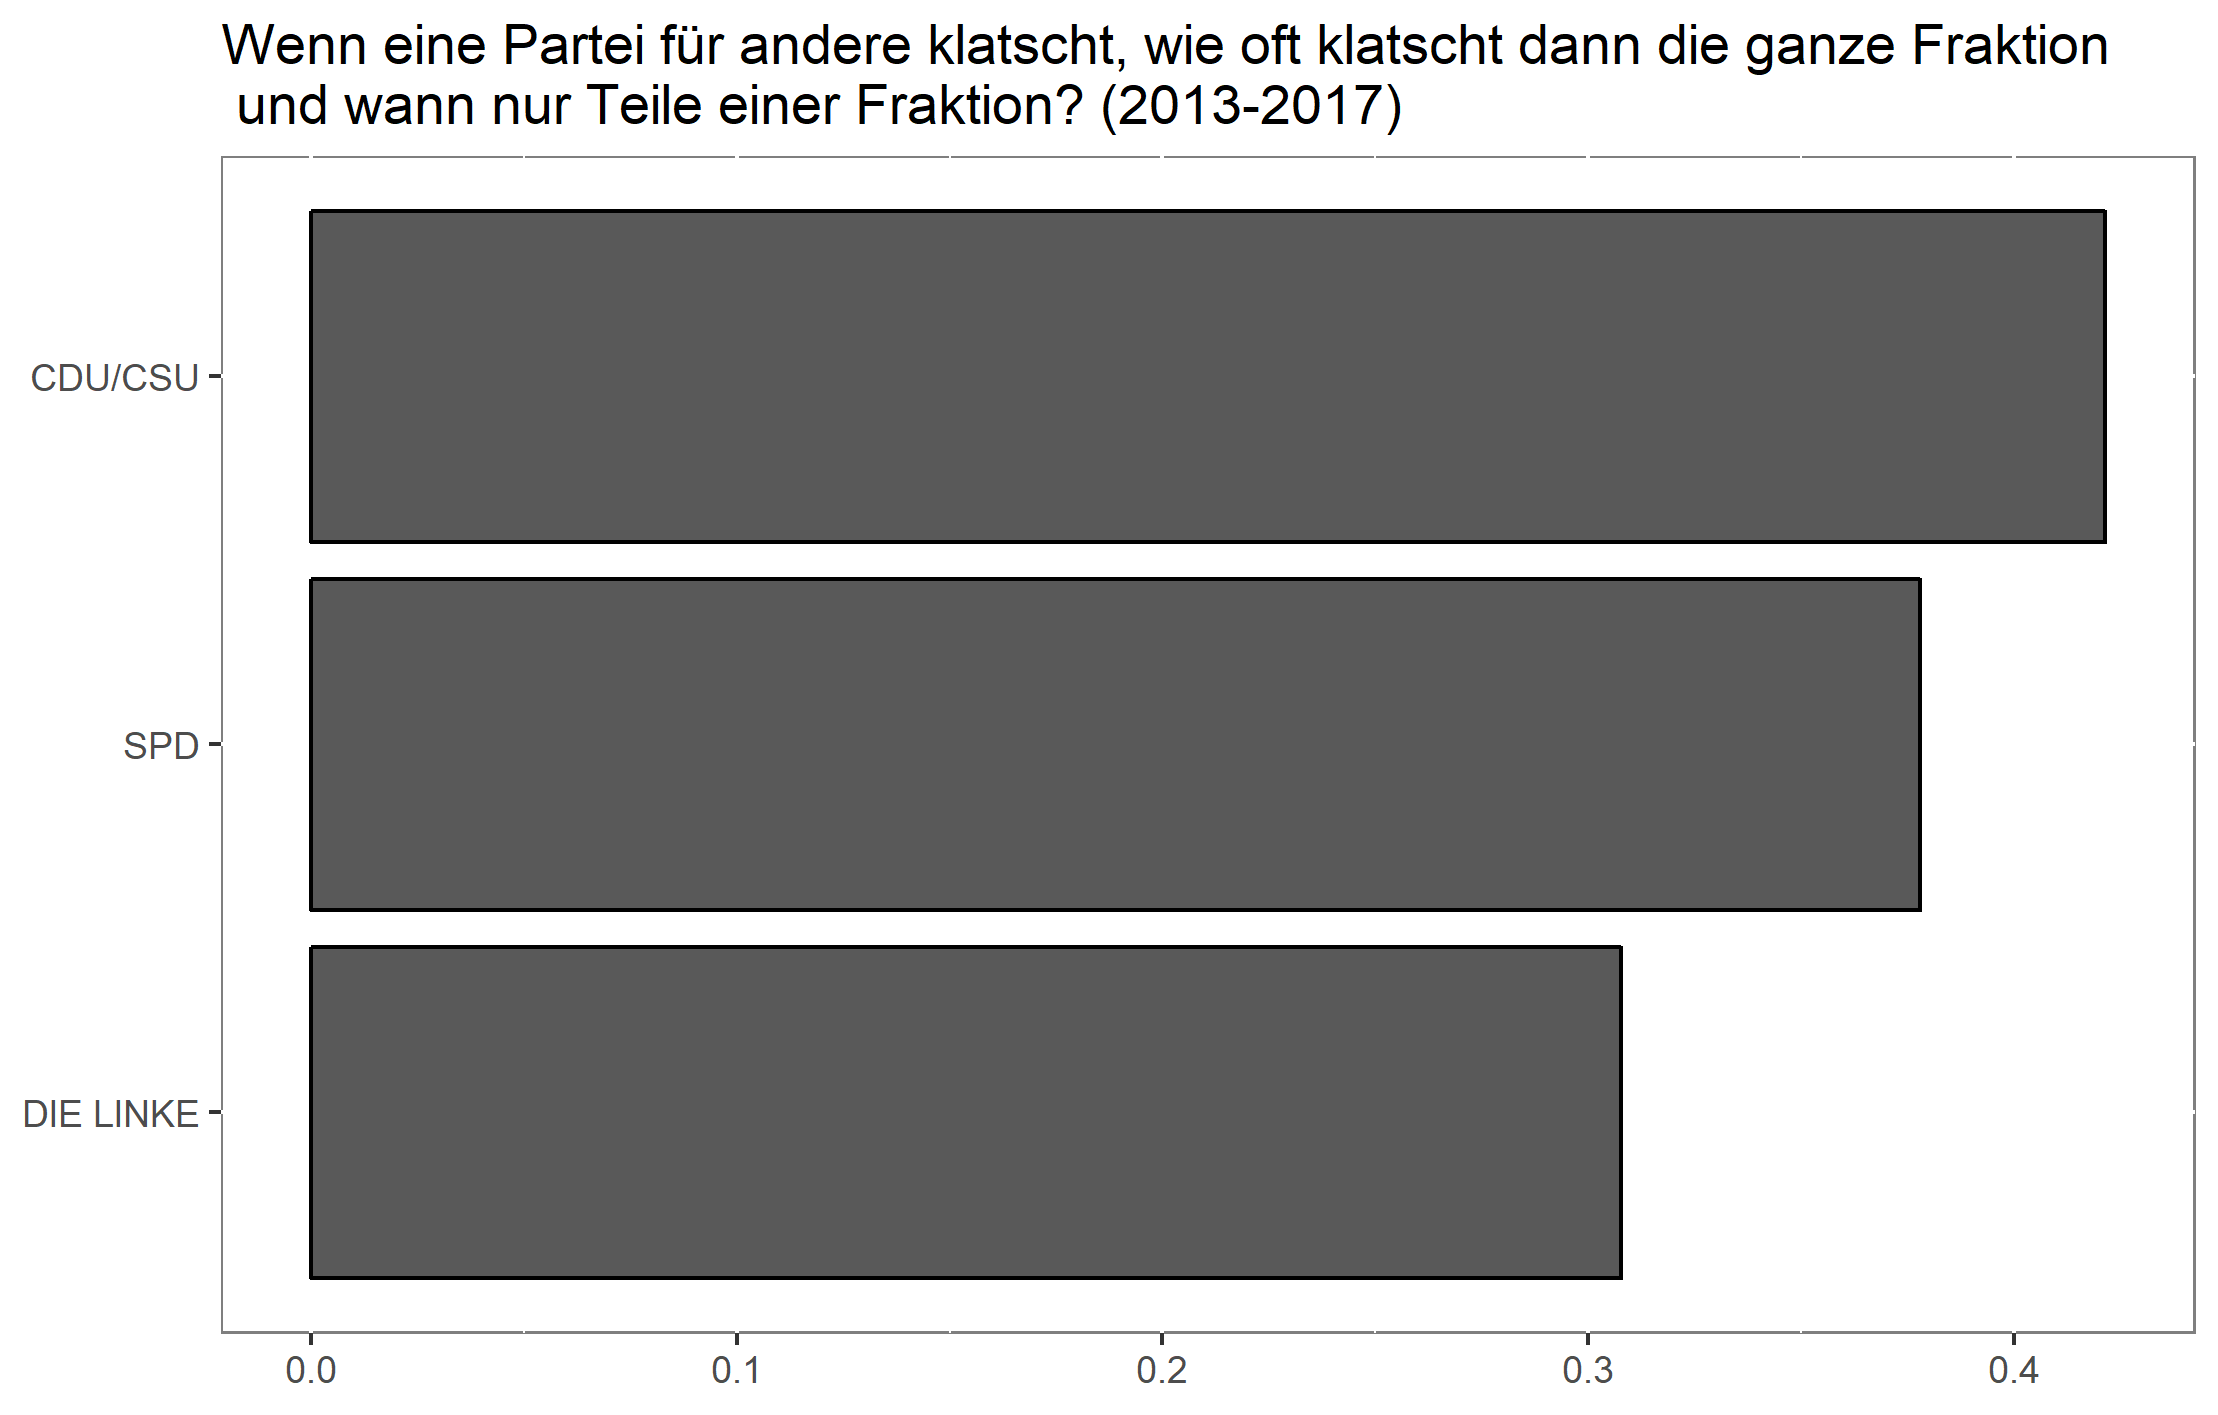
\includegraphics[width=\linewidth]{Grafiken/Geschlossenheit13.png}
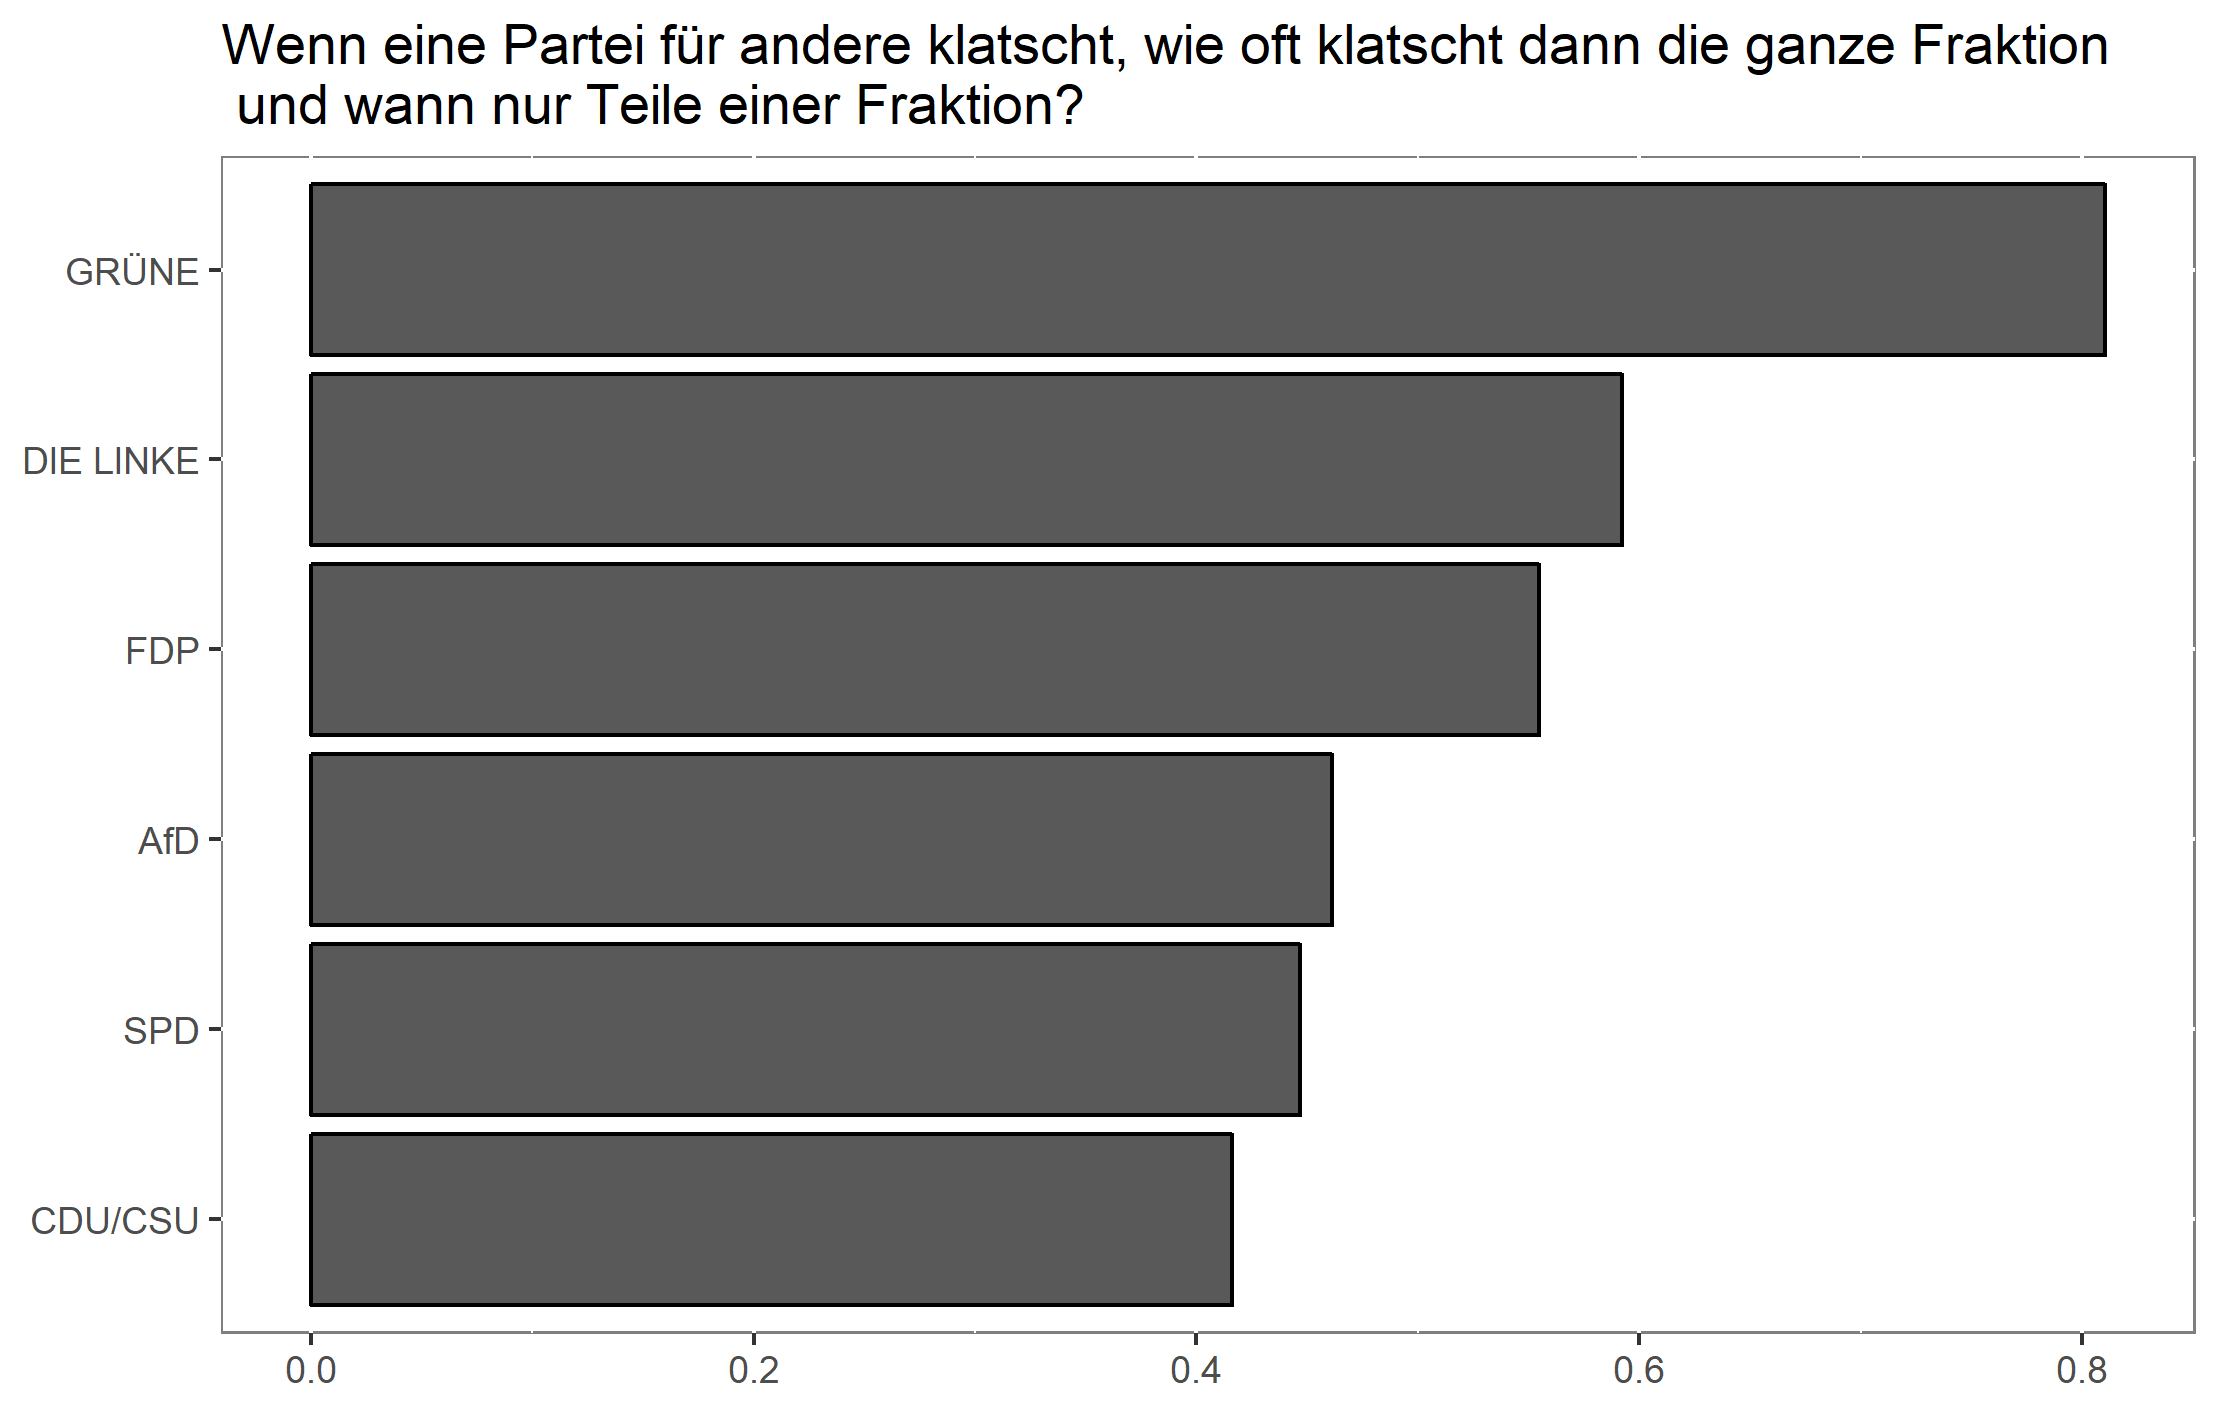
\includegraphics[width=\linewidth]{Grafiken/Geschlossenheit17.png}\\

Es zeigt sich, dass weder die Hypothese bestätigt werden kann, dass sich eine große Veränderung bezüglich der Geschlossenheit gegeben hat, noch, dass die AfD als Newcomer-Partei weder besonders geschlossen, noch besonders gespalten auftritt. Interessanter ist eher, dass sich der Fraktionsstreit der CDU mit der CSU deutlich in dem Ergebniss zeigt, dass die CDU/CSU plötzlich auf dem letzten Platz ist und in fast der Hälfte der Fälle nur einzelne Abgeordnete Klatschen und nicht die ganze Partei. 

\subsubsection{Isolierung in der Wortwahl} 
Die Grafik spricht für sich. Die einzige Partei, die "Deutschland und deutsch" häufiger verwendet, als "Mensch" ist die AfD. \\

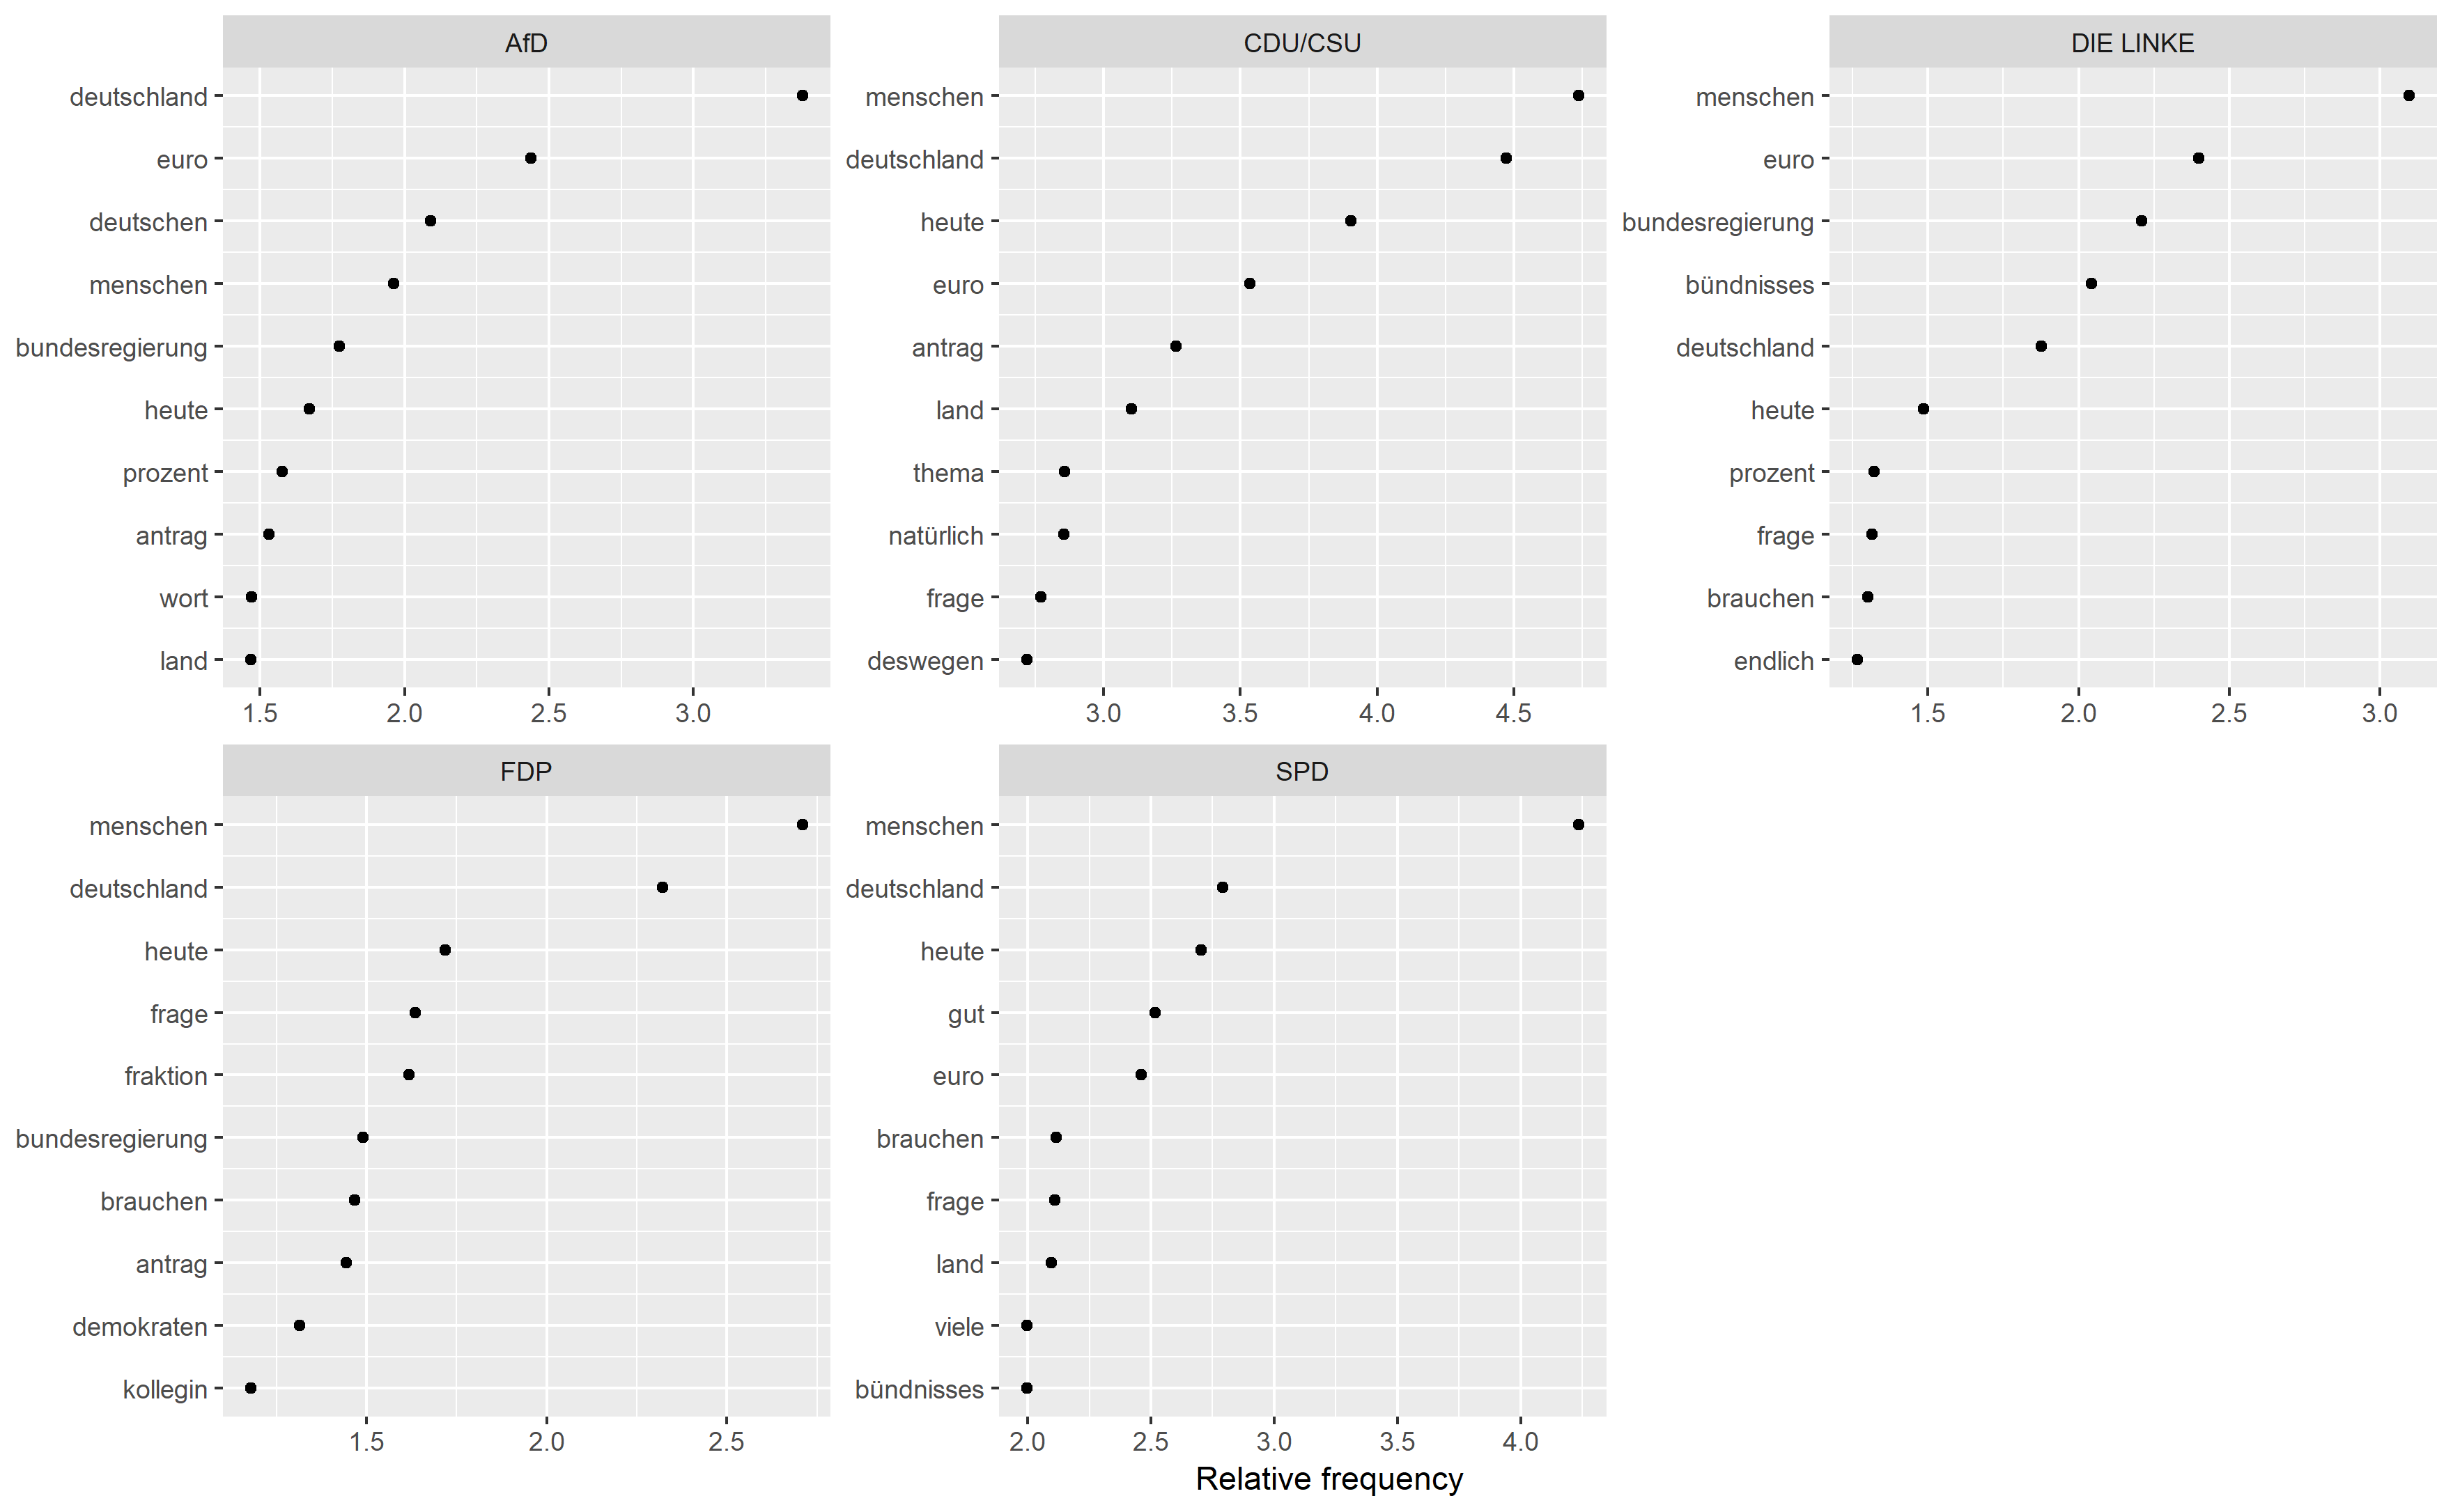
\includegraphics[width=\linewidth]{Grafiken/17_HäufigsteWörter.png}\\

\subsection{Negative Interaktionen}

"Lachen" wird vom stenografischen Dienst in Abgrenzung zur "Heiterkeit" als negative, Aktion beschrieben. Ebenso wird "Widerspruch" und "Zuruf", in Abgrenzung zu einem Kommentar, der sowohl positiv, als auch negativ sein kann, als negative Aktion beschrieben. 

%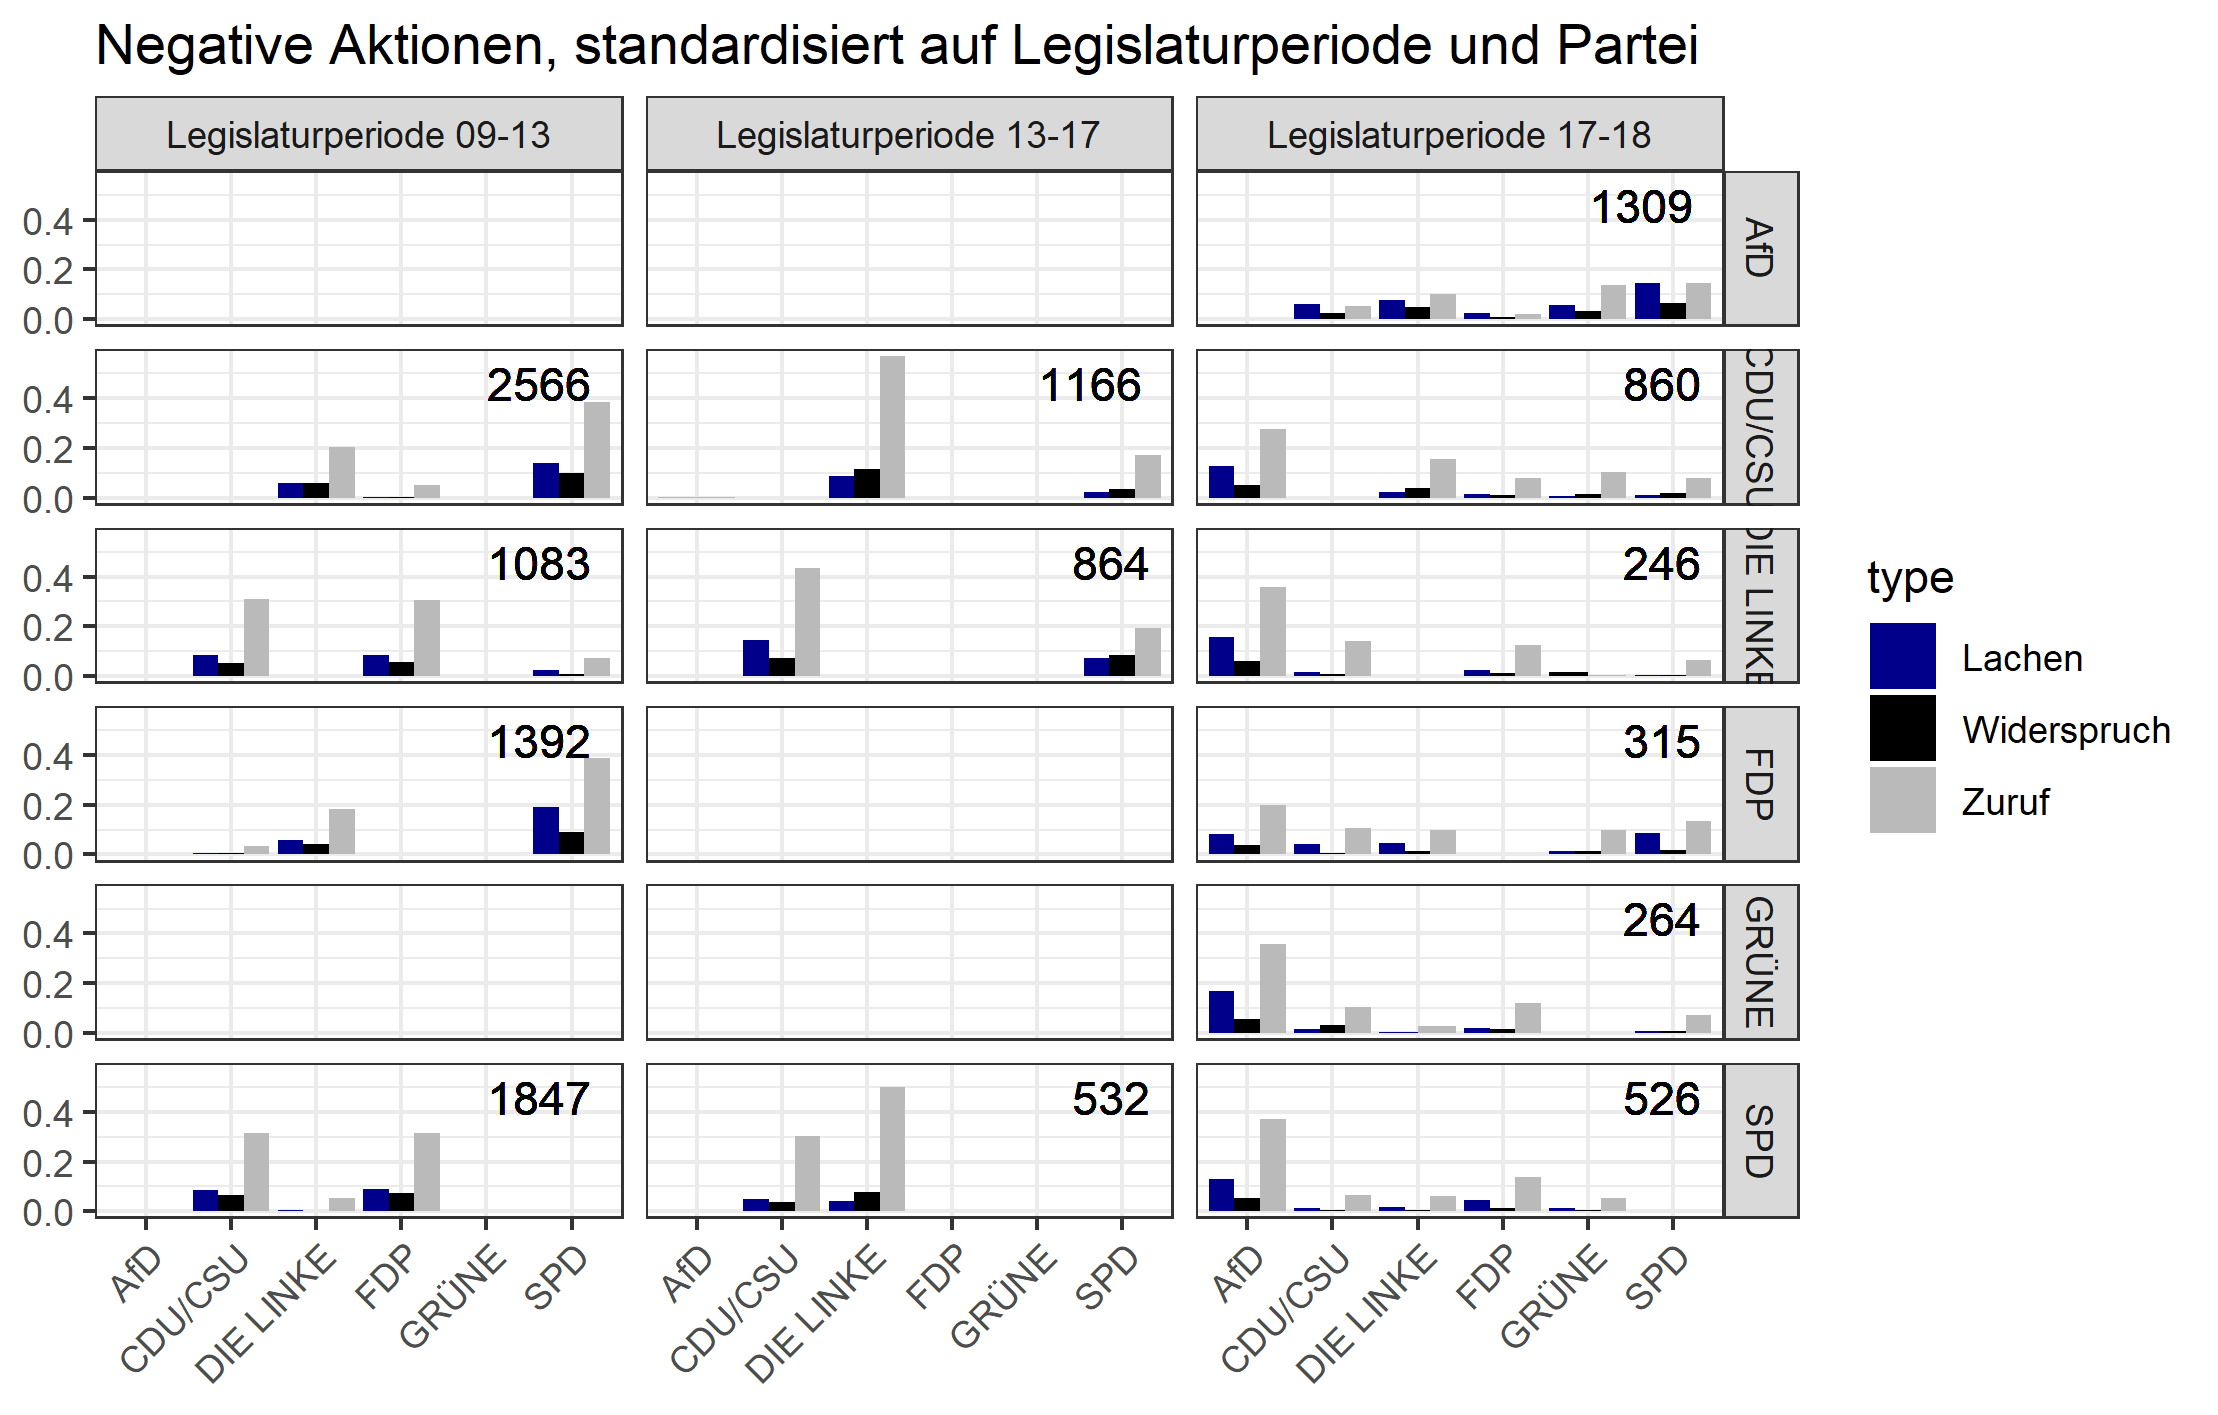
\includegraphics[width=\linewidth]{Grafiken/WelchePArteiLachtwieviel.png}

Unsere Vermutung, dass die AfD am häufigsten Lacht ist damit bestätigt. 

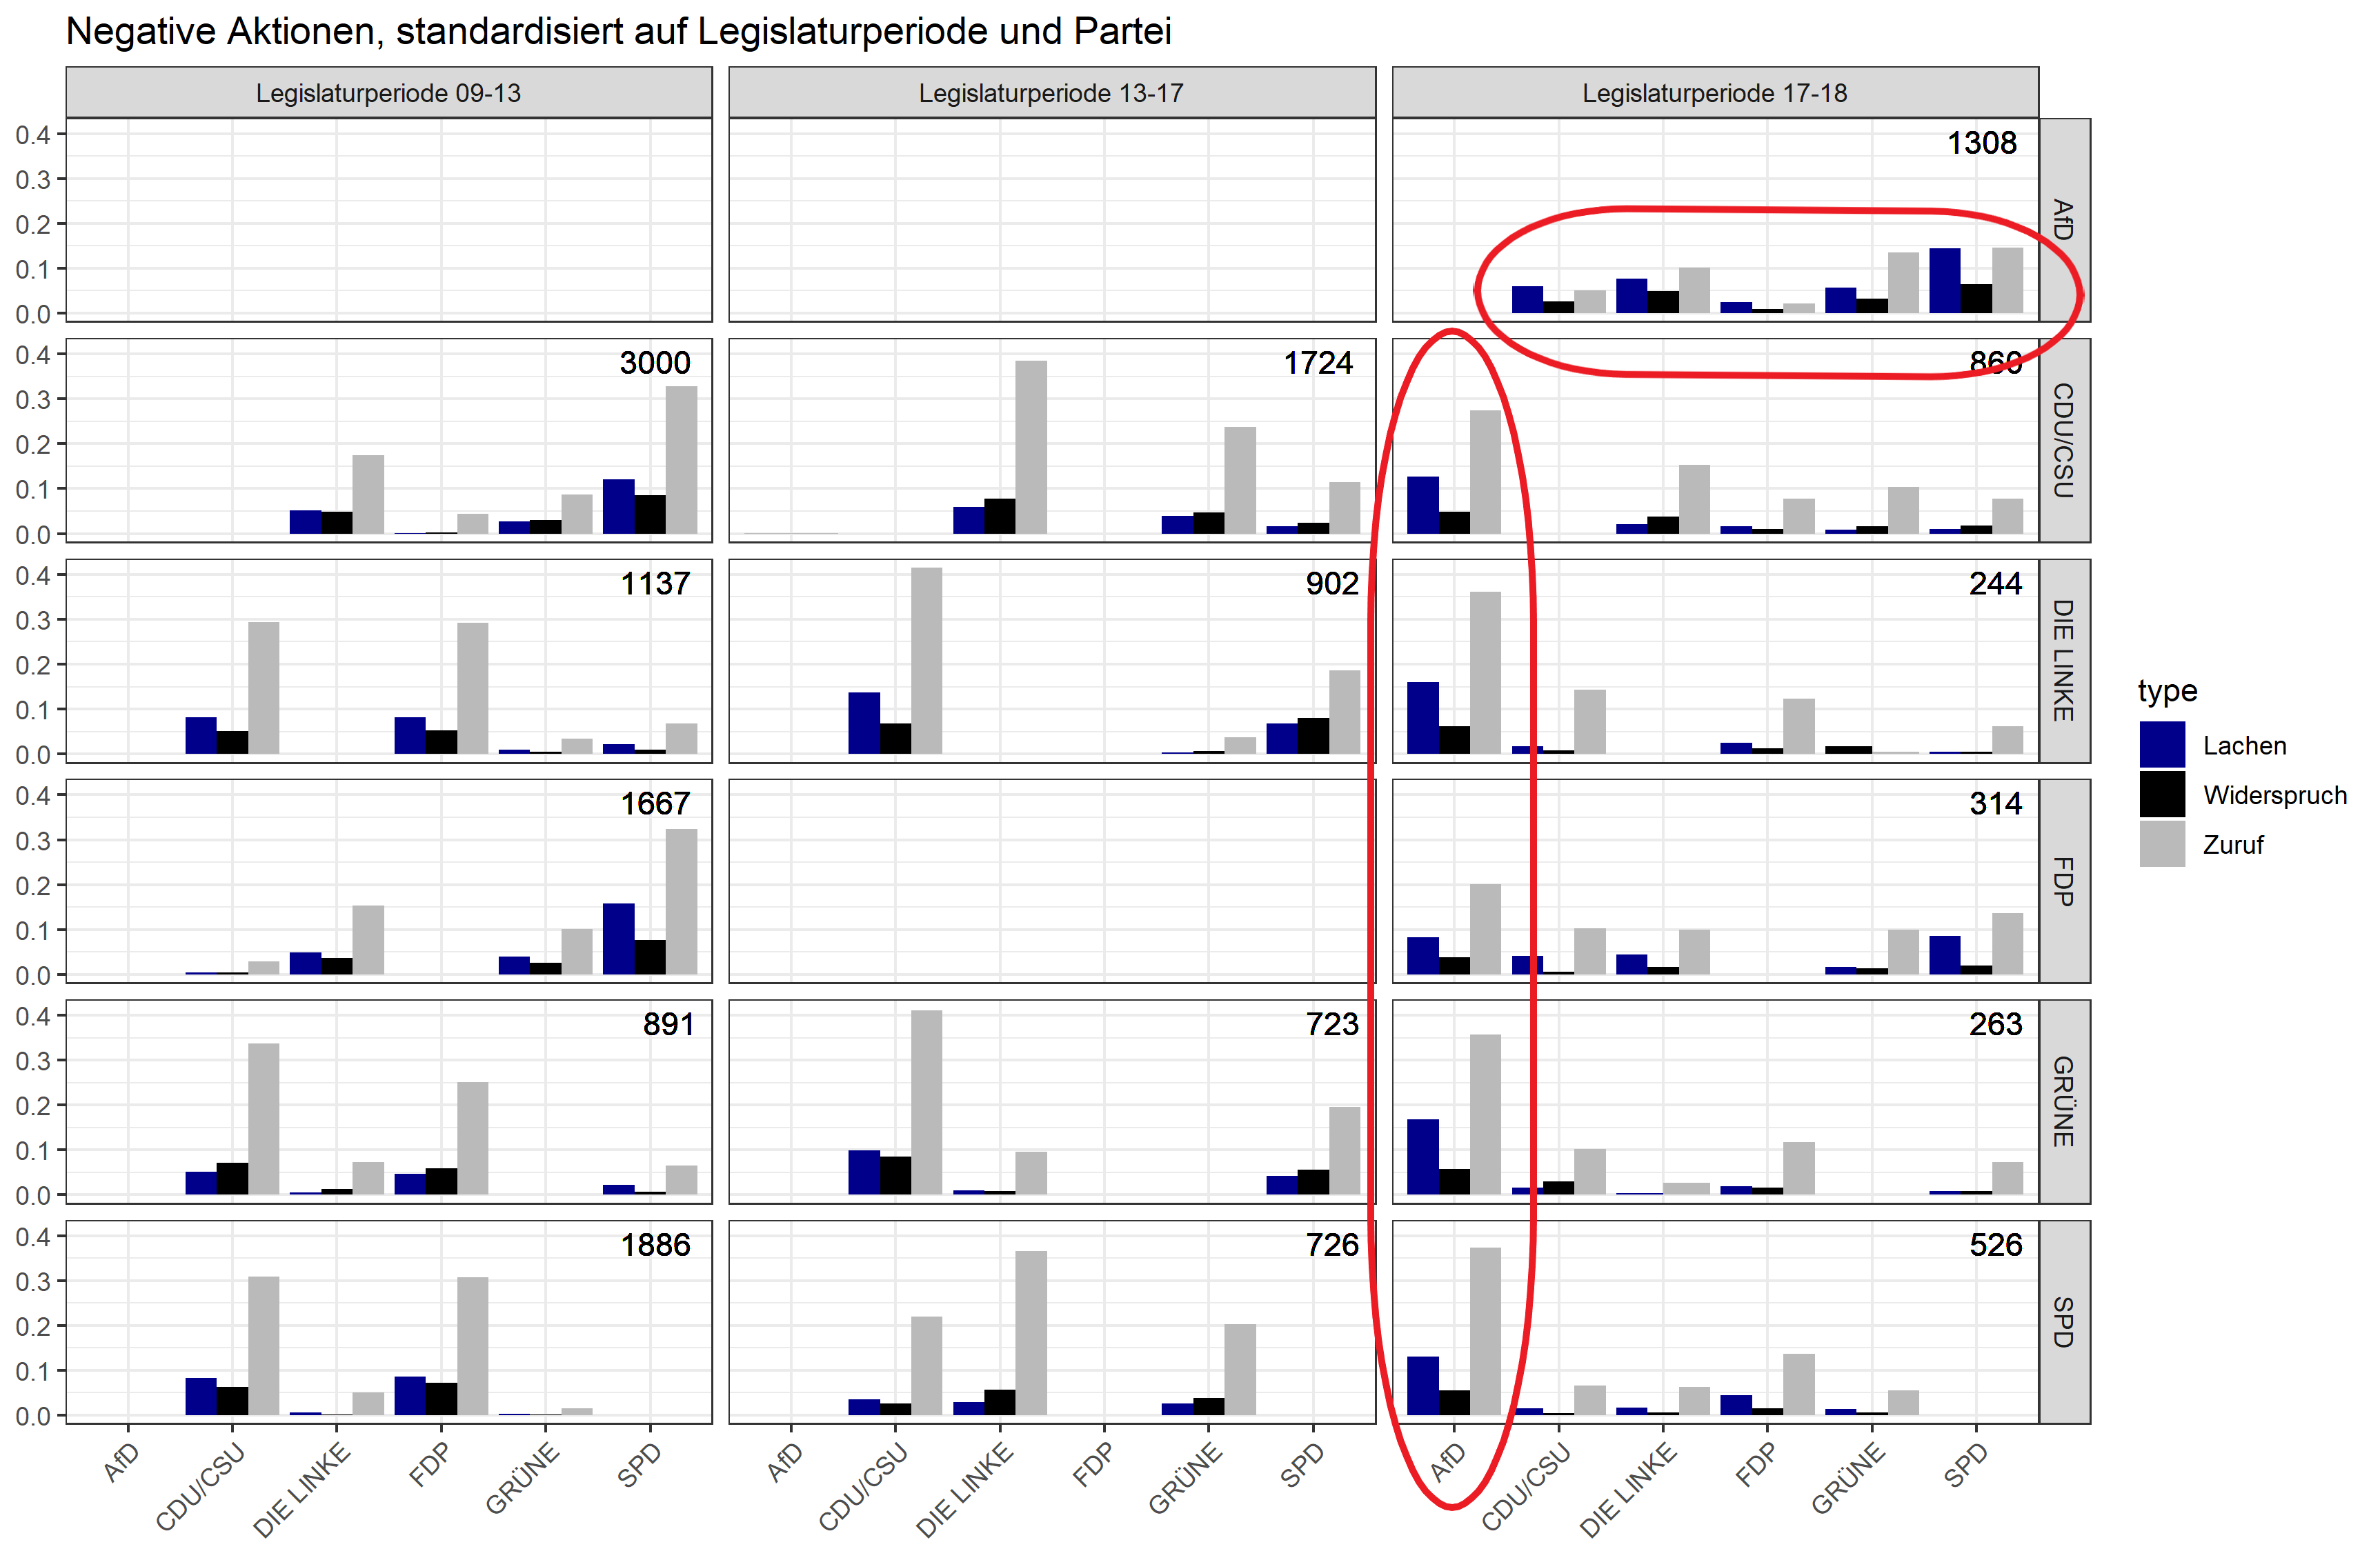
\includegraphics[width=\linewidth]{Grafiken/13_17negativ_perc_bunt.png}\\

%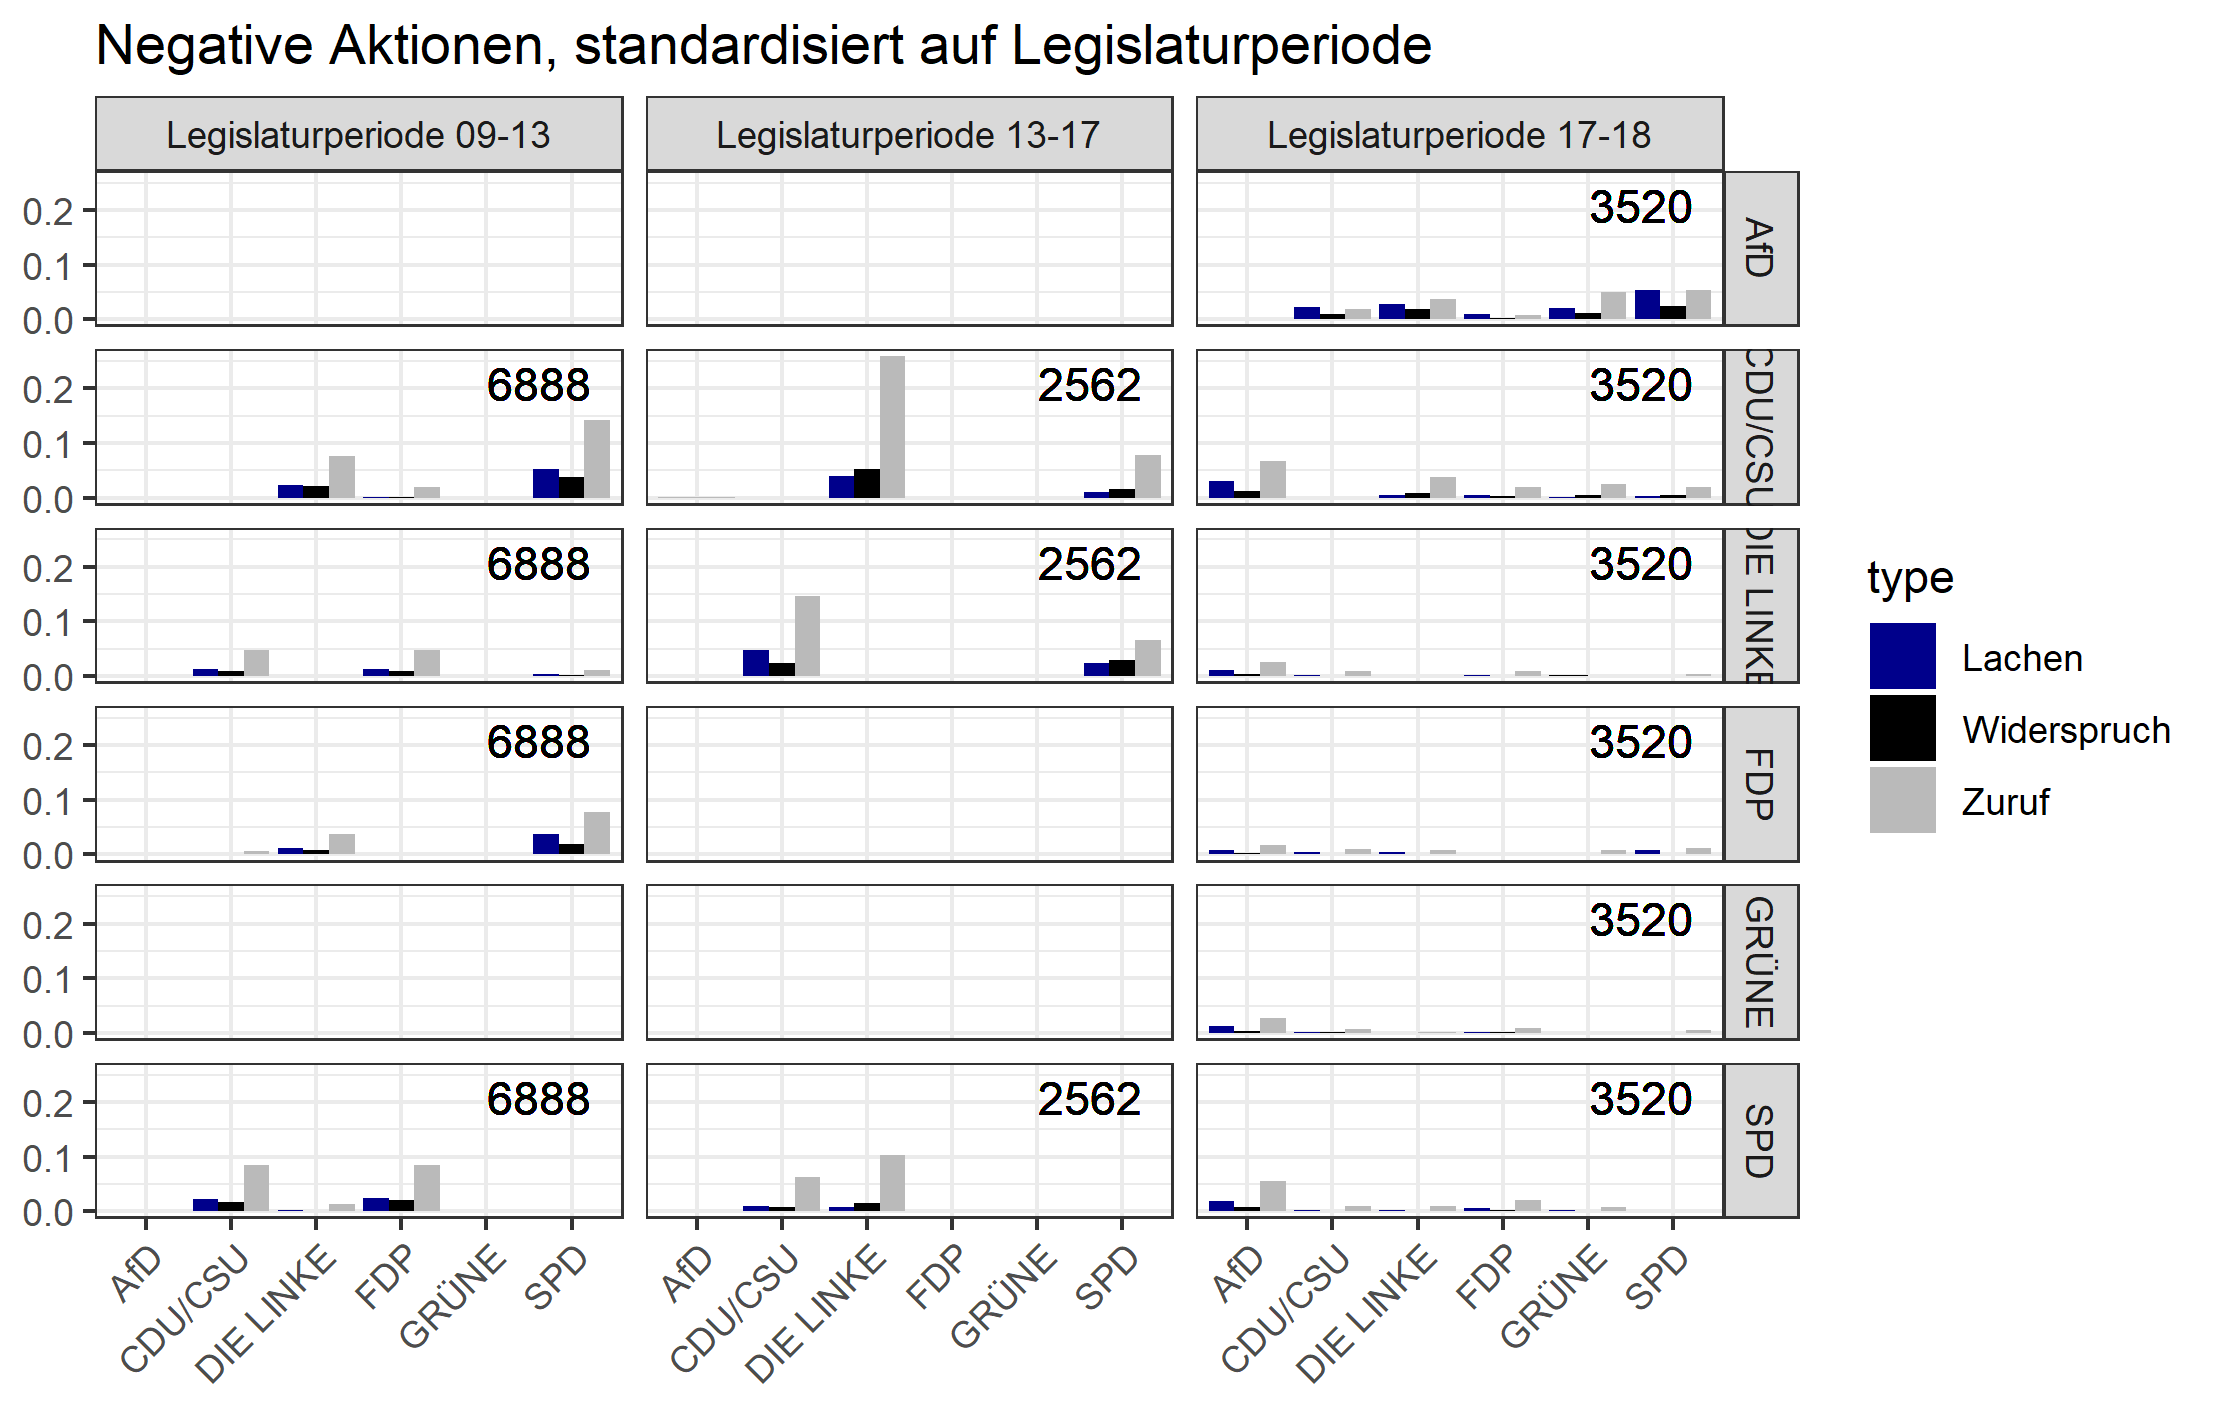
\includegraphics[width=\linewidth]{Grafiken/13_17negativ_leg.png}\\
%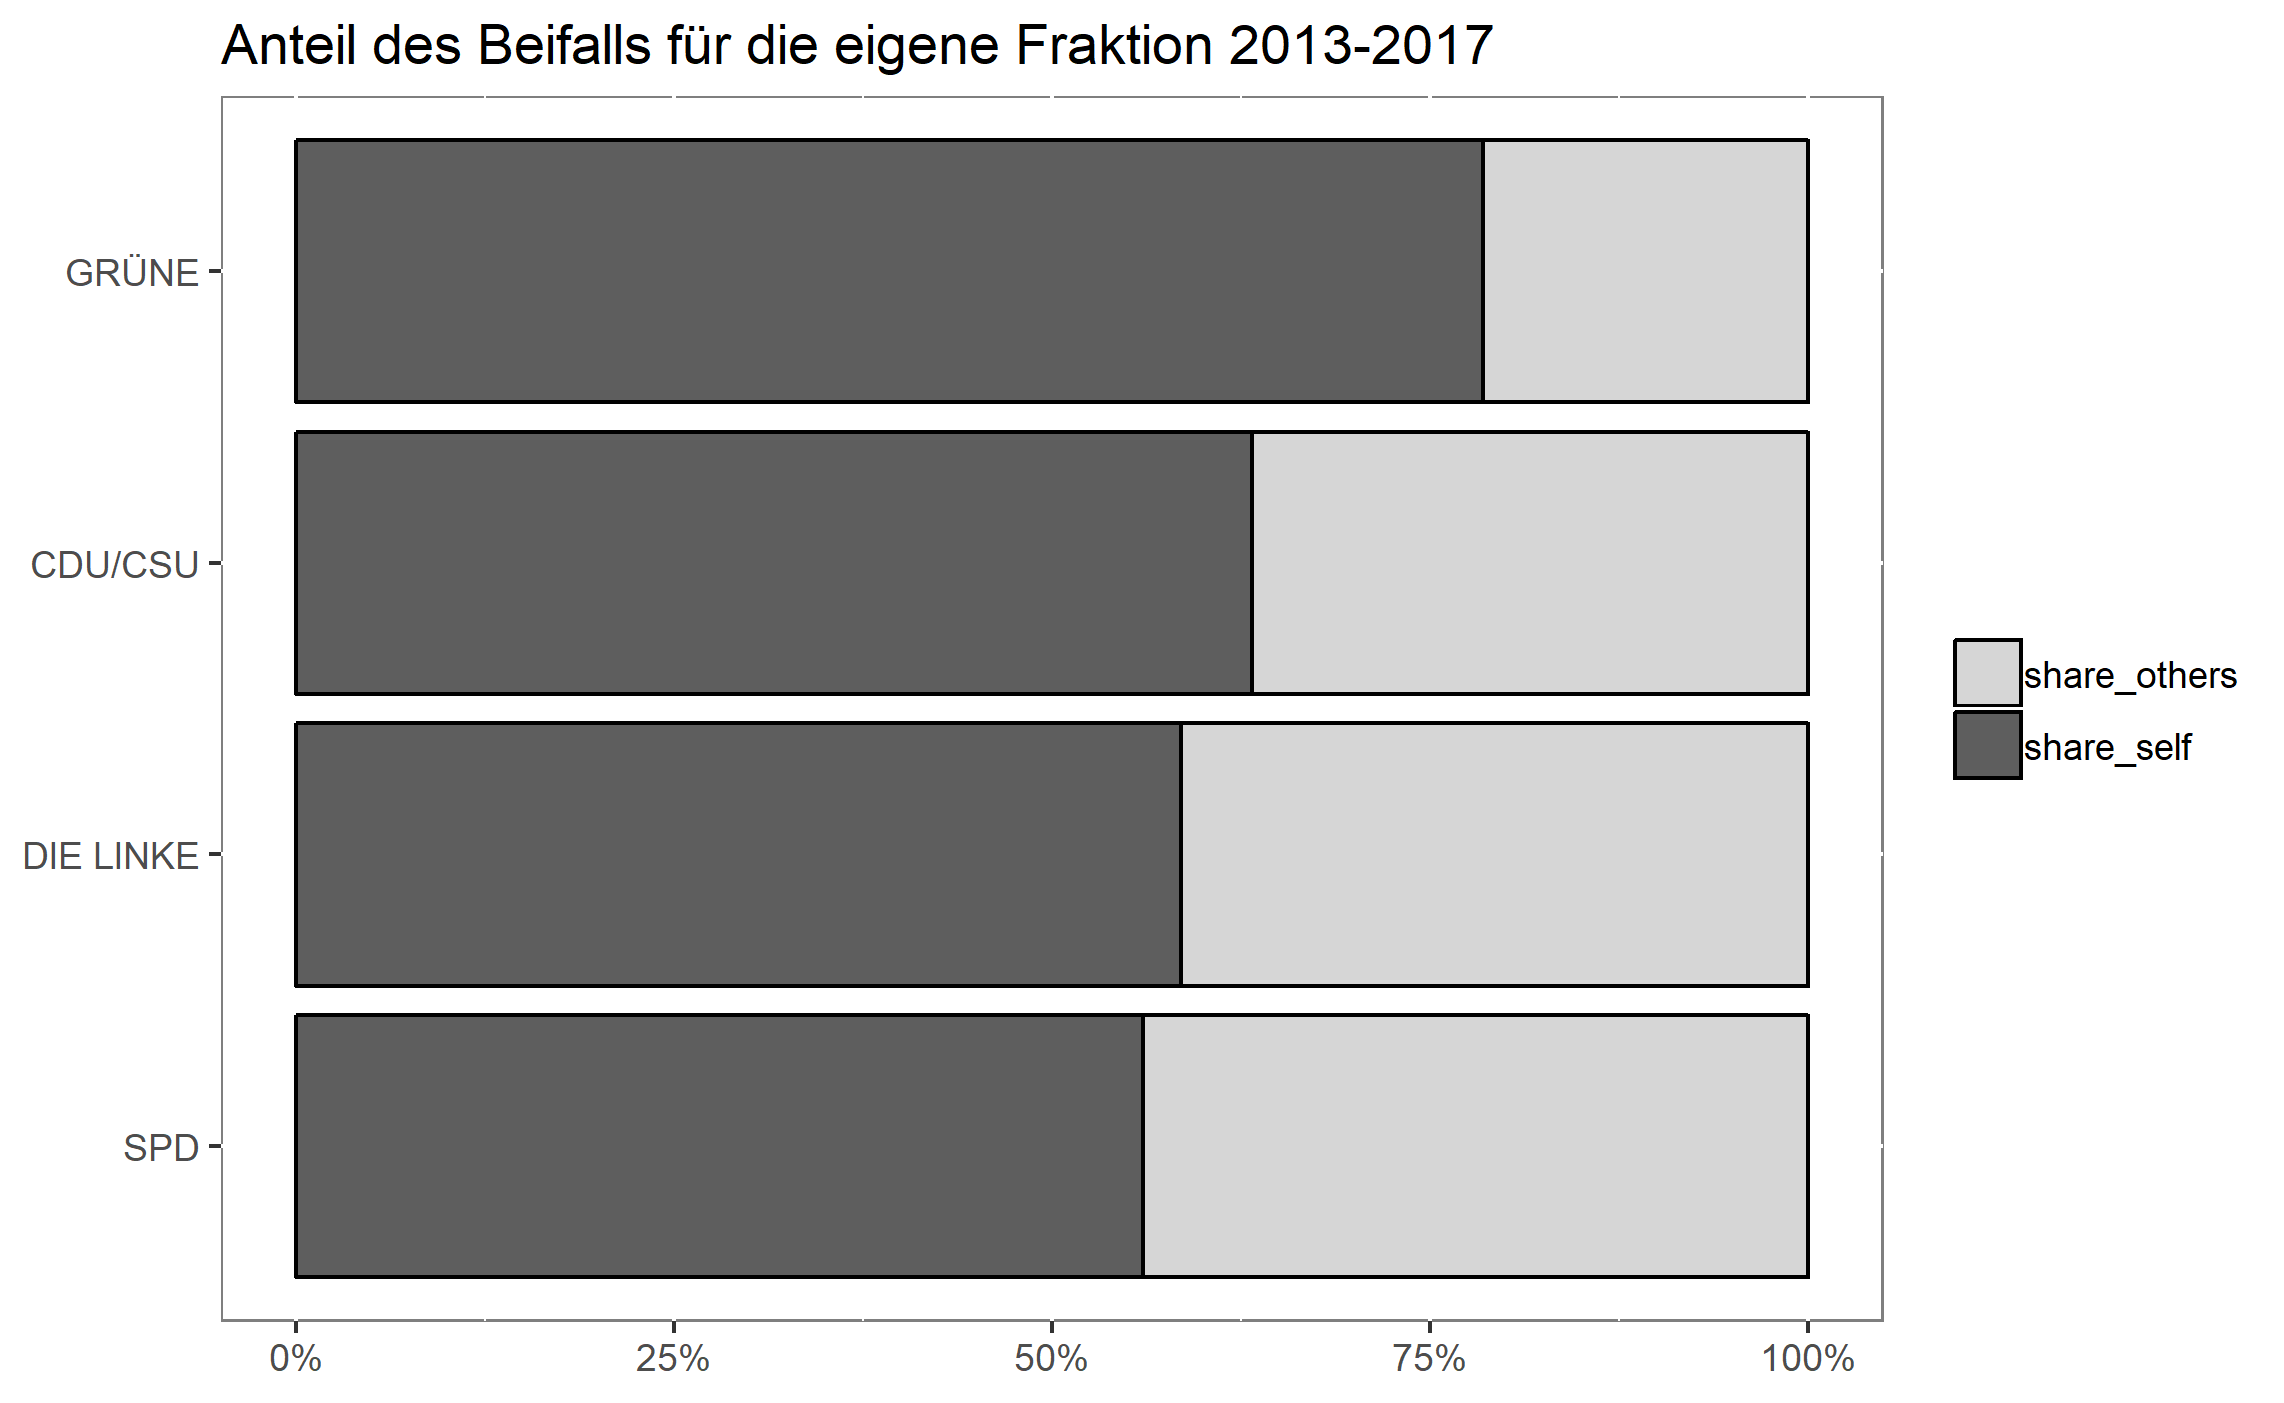
\includegraphics[width=\linewidth]{Grafiken/13_eigenklatschanteil.png}







\subsection {Readability Index}
Der Flesch-Reading Index, der auf englische Texte optimiert
ist wurde von Amstad (\cite{amstad_wie_1978}) auf deutsprachige Texte angepasst. Die
Werte wurden mit der Funktion \texttt{flesch()} mit dem Parameter {\verb de } aus dem R-Package KoRpus (\cite{michalke_korpus:_2018}) berechnet.\\

\fbox{\parbox{\linewidth}{\[r_{German} = 80 - 58.5 * \frac{x}{y} - \frac{w}{s} \] \textbf{w}: Gesamtanzahl von Wörtern \textbf{y}: Gesamtanzahl von Silben \textbf{s}: Gesamtanzahl von Sätzen}}\\


\noindent Dafür wurden die Texte zunächst in Buchstaben aufgeteilt. Dies wurde mit
der \texttt{tokenize()} funktion aus dem ``koRpus'' Package gemacht.

\begin{longtable}[]{@{}lll@{}}
	\toprule
	Flesch-Reading-Ease-Score Von \ldots{} bis unter \ldots{} & Lesbarkeit &
	Verständlich für\tabularnewline
	\midrule
	\endhead
	0--30 & Sehr schwer & Akademiker\tabularnewline
	30--50 & Schwer &\tabularnewline
	50--60 & Mittelschwer &\tabularnewline
	60--70 & Mittel & 13--15-jährige Schüler\tabularnewline
	70--80 & Mittelleicht &\tabularnewline
	80--90 & Leicht &\tabularnewline
	90--100 & Sehr leicht & 11-jährige Schüler\tabularnewline
	\bottomrule
\end{longtable}


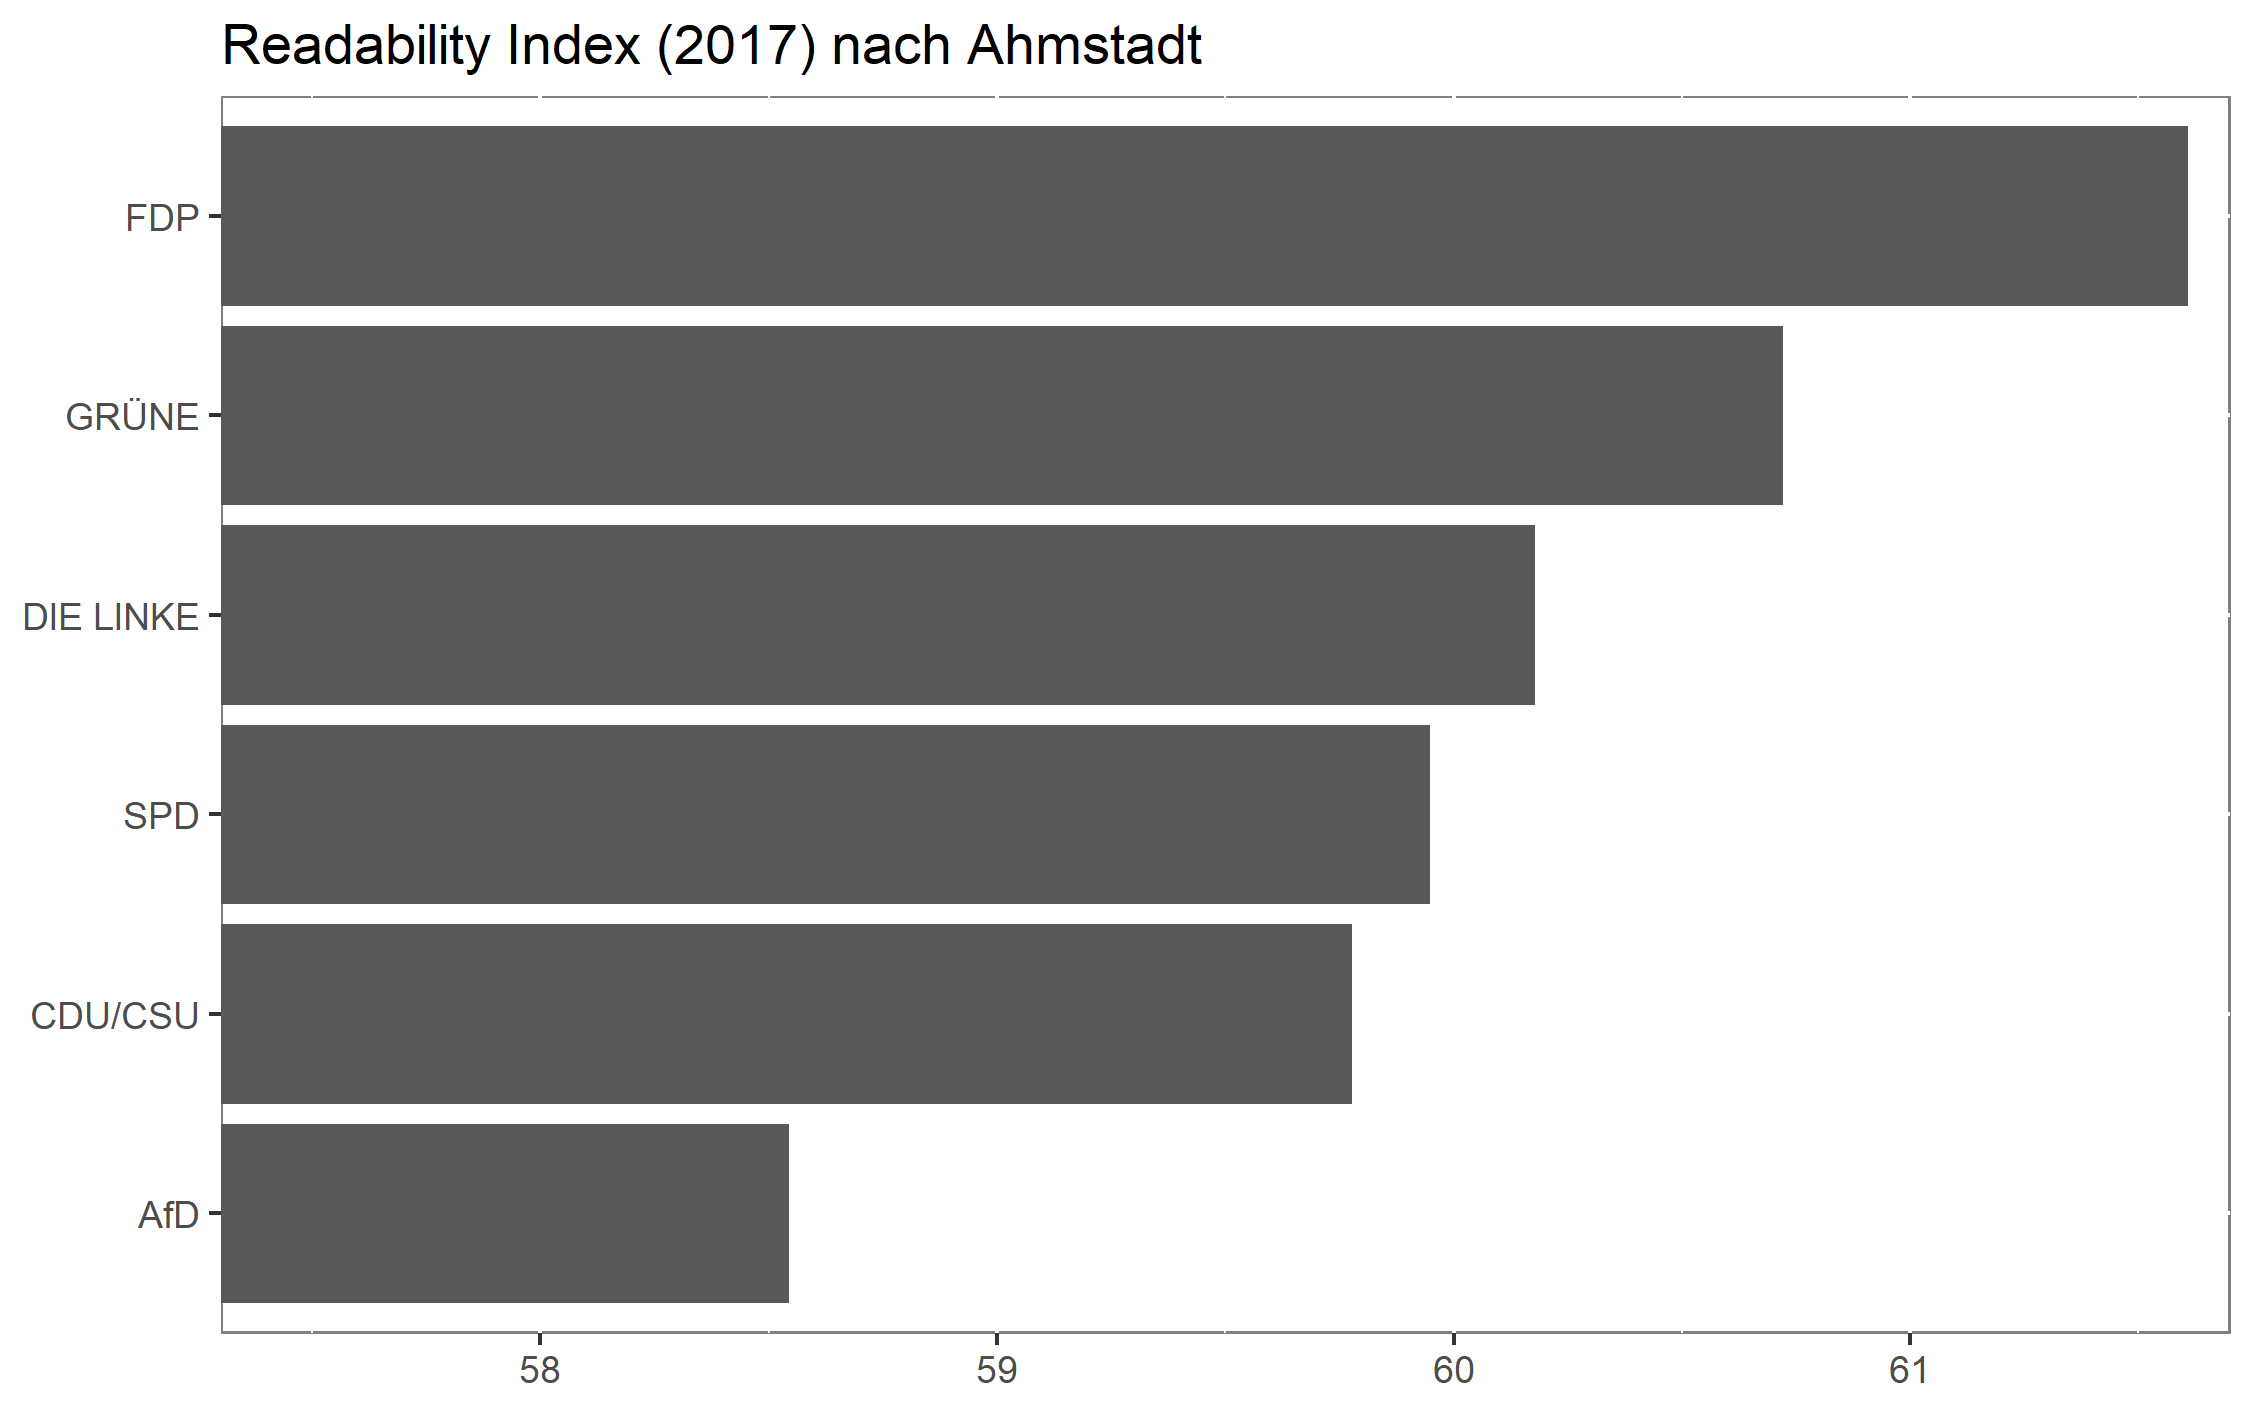
\includegraphics[width=\linewidth]{Grafiken/Readability_line.png}\\

Die Hypothese kann nicht bestätigt werden. Eine Aufschlüsselung des
Lesbarkeitsindex nach Politikern könnte in weiter Forschung dennoch Aufschluss über
Veränderungen auf personaler Ebene geben.\\
\newpage

\subsection{Die Inhalte sind seit dem Einzug der AfD einseitiger geworden}

Hypothese kann verworfen werden. Die Themen sind sogar eher gleicher verteilt. 

\begin{figure} [h]
	\subfigure[2009]{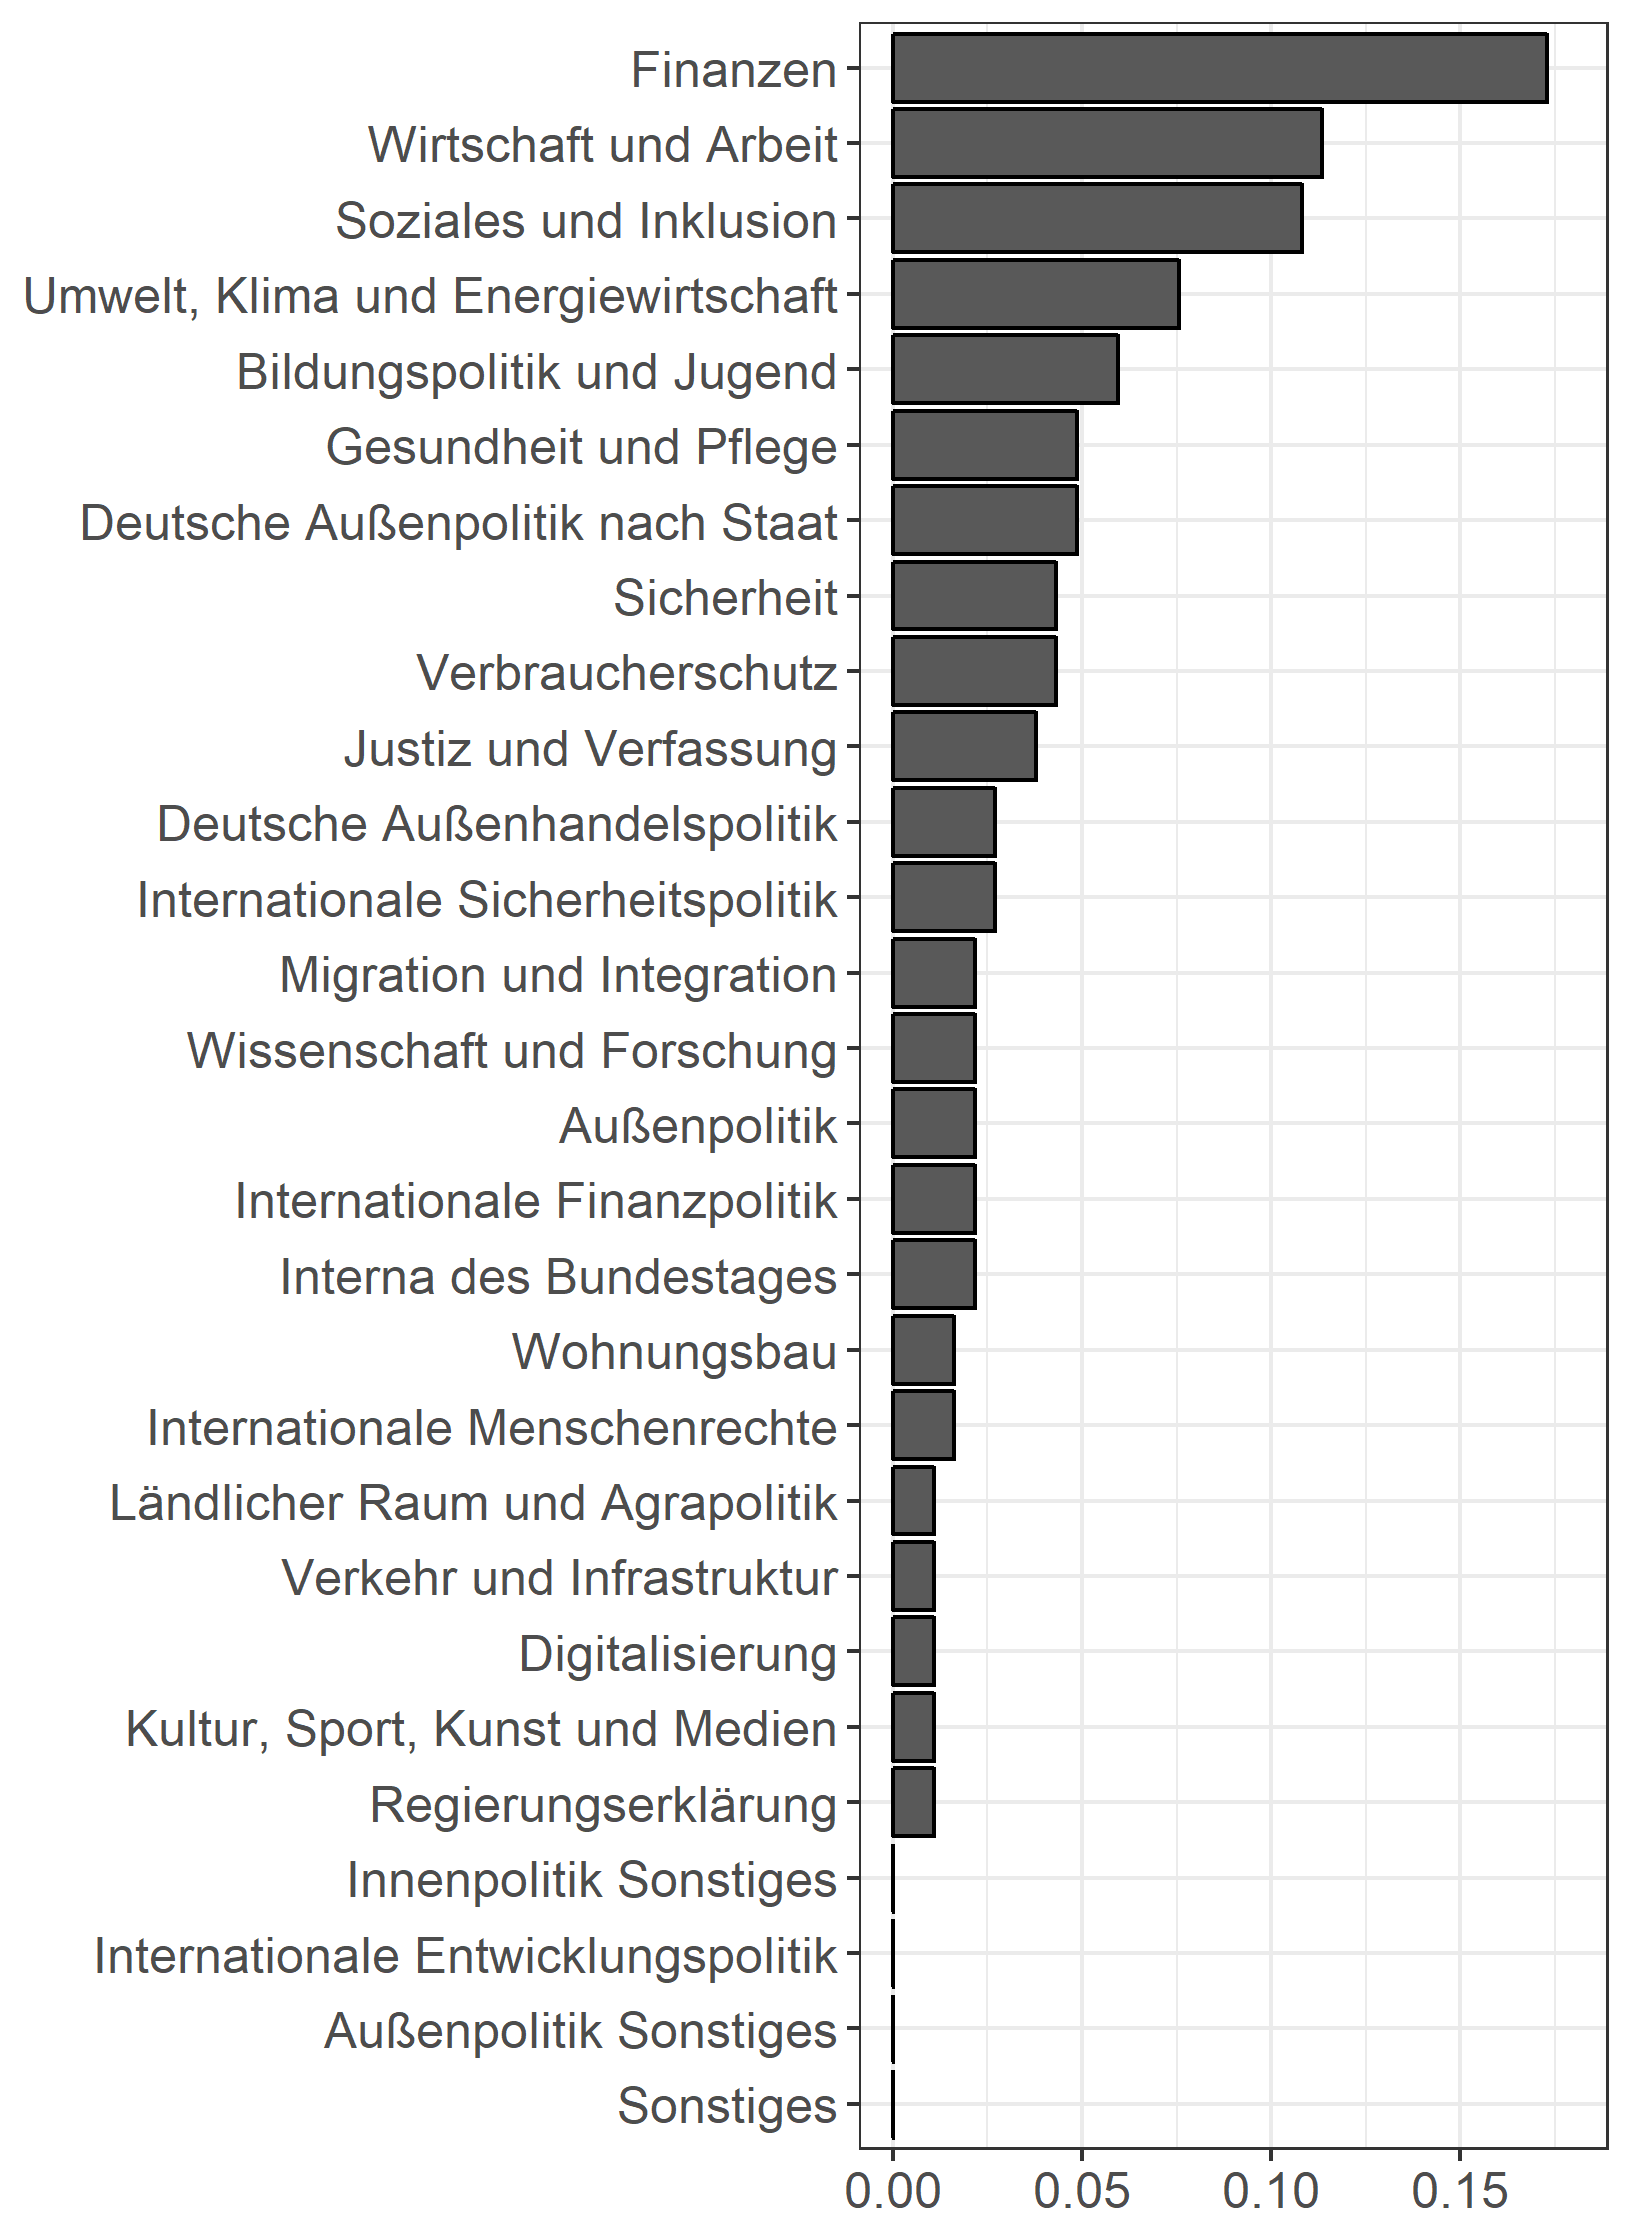
\includegraphics[width=0.29\textwidth]{Grafiken/Inhalt09.png}}
	\subfigure[2013]{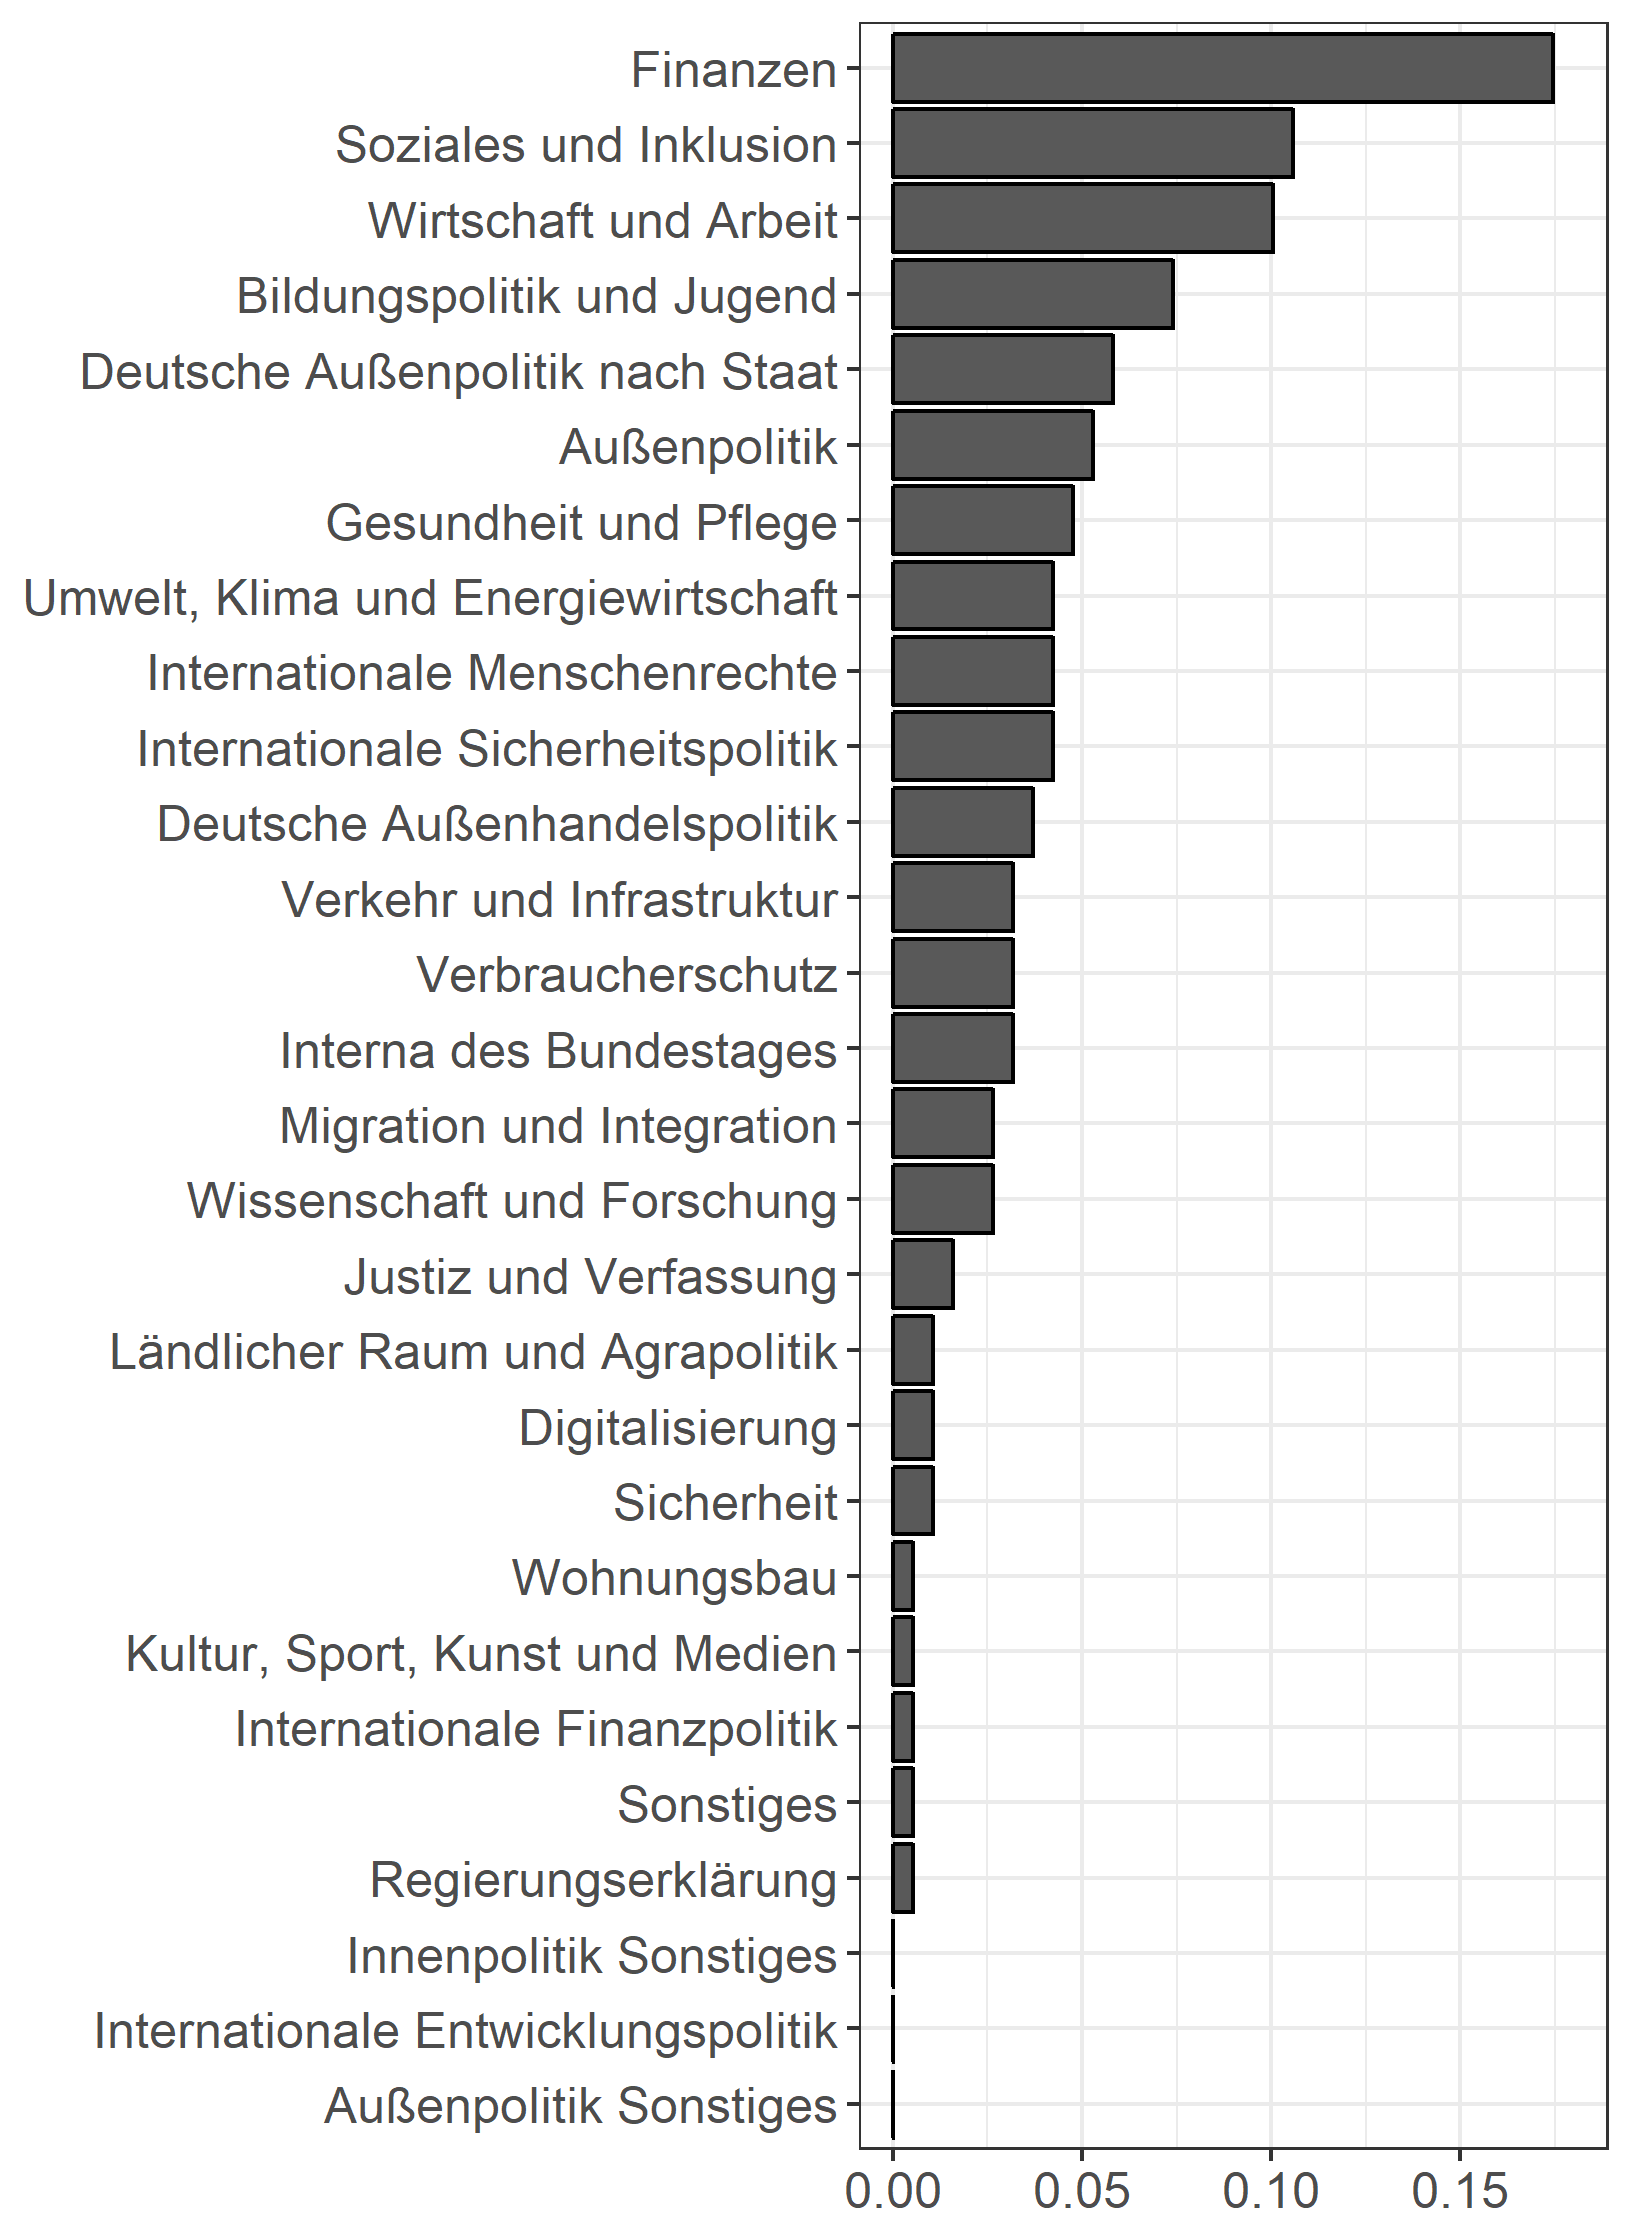
\includegraphics[width=0.29\textwidth]{Grafiken/Inhalt13.png}}
	\subfigure[2017]{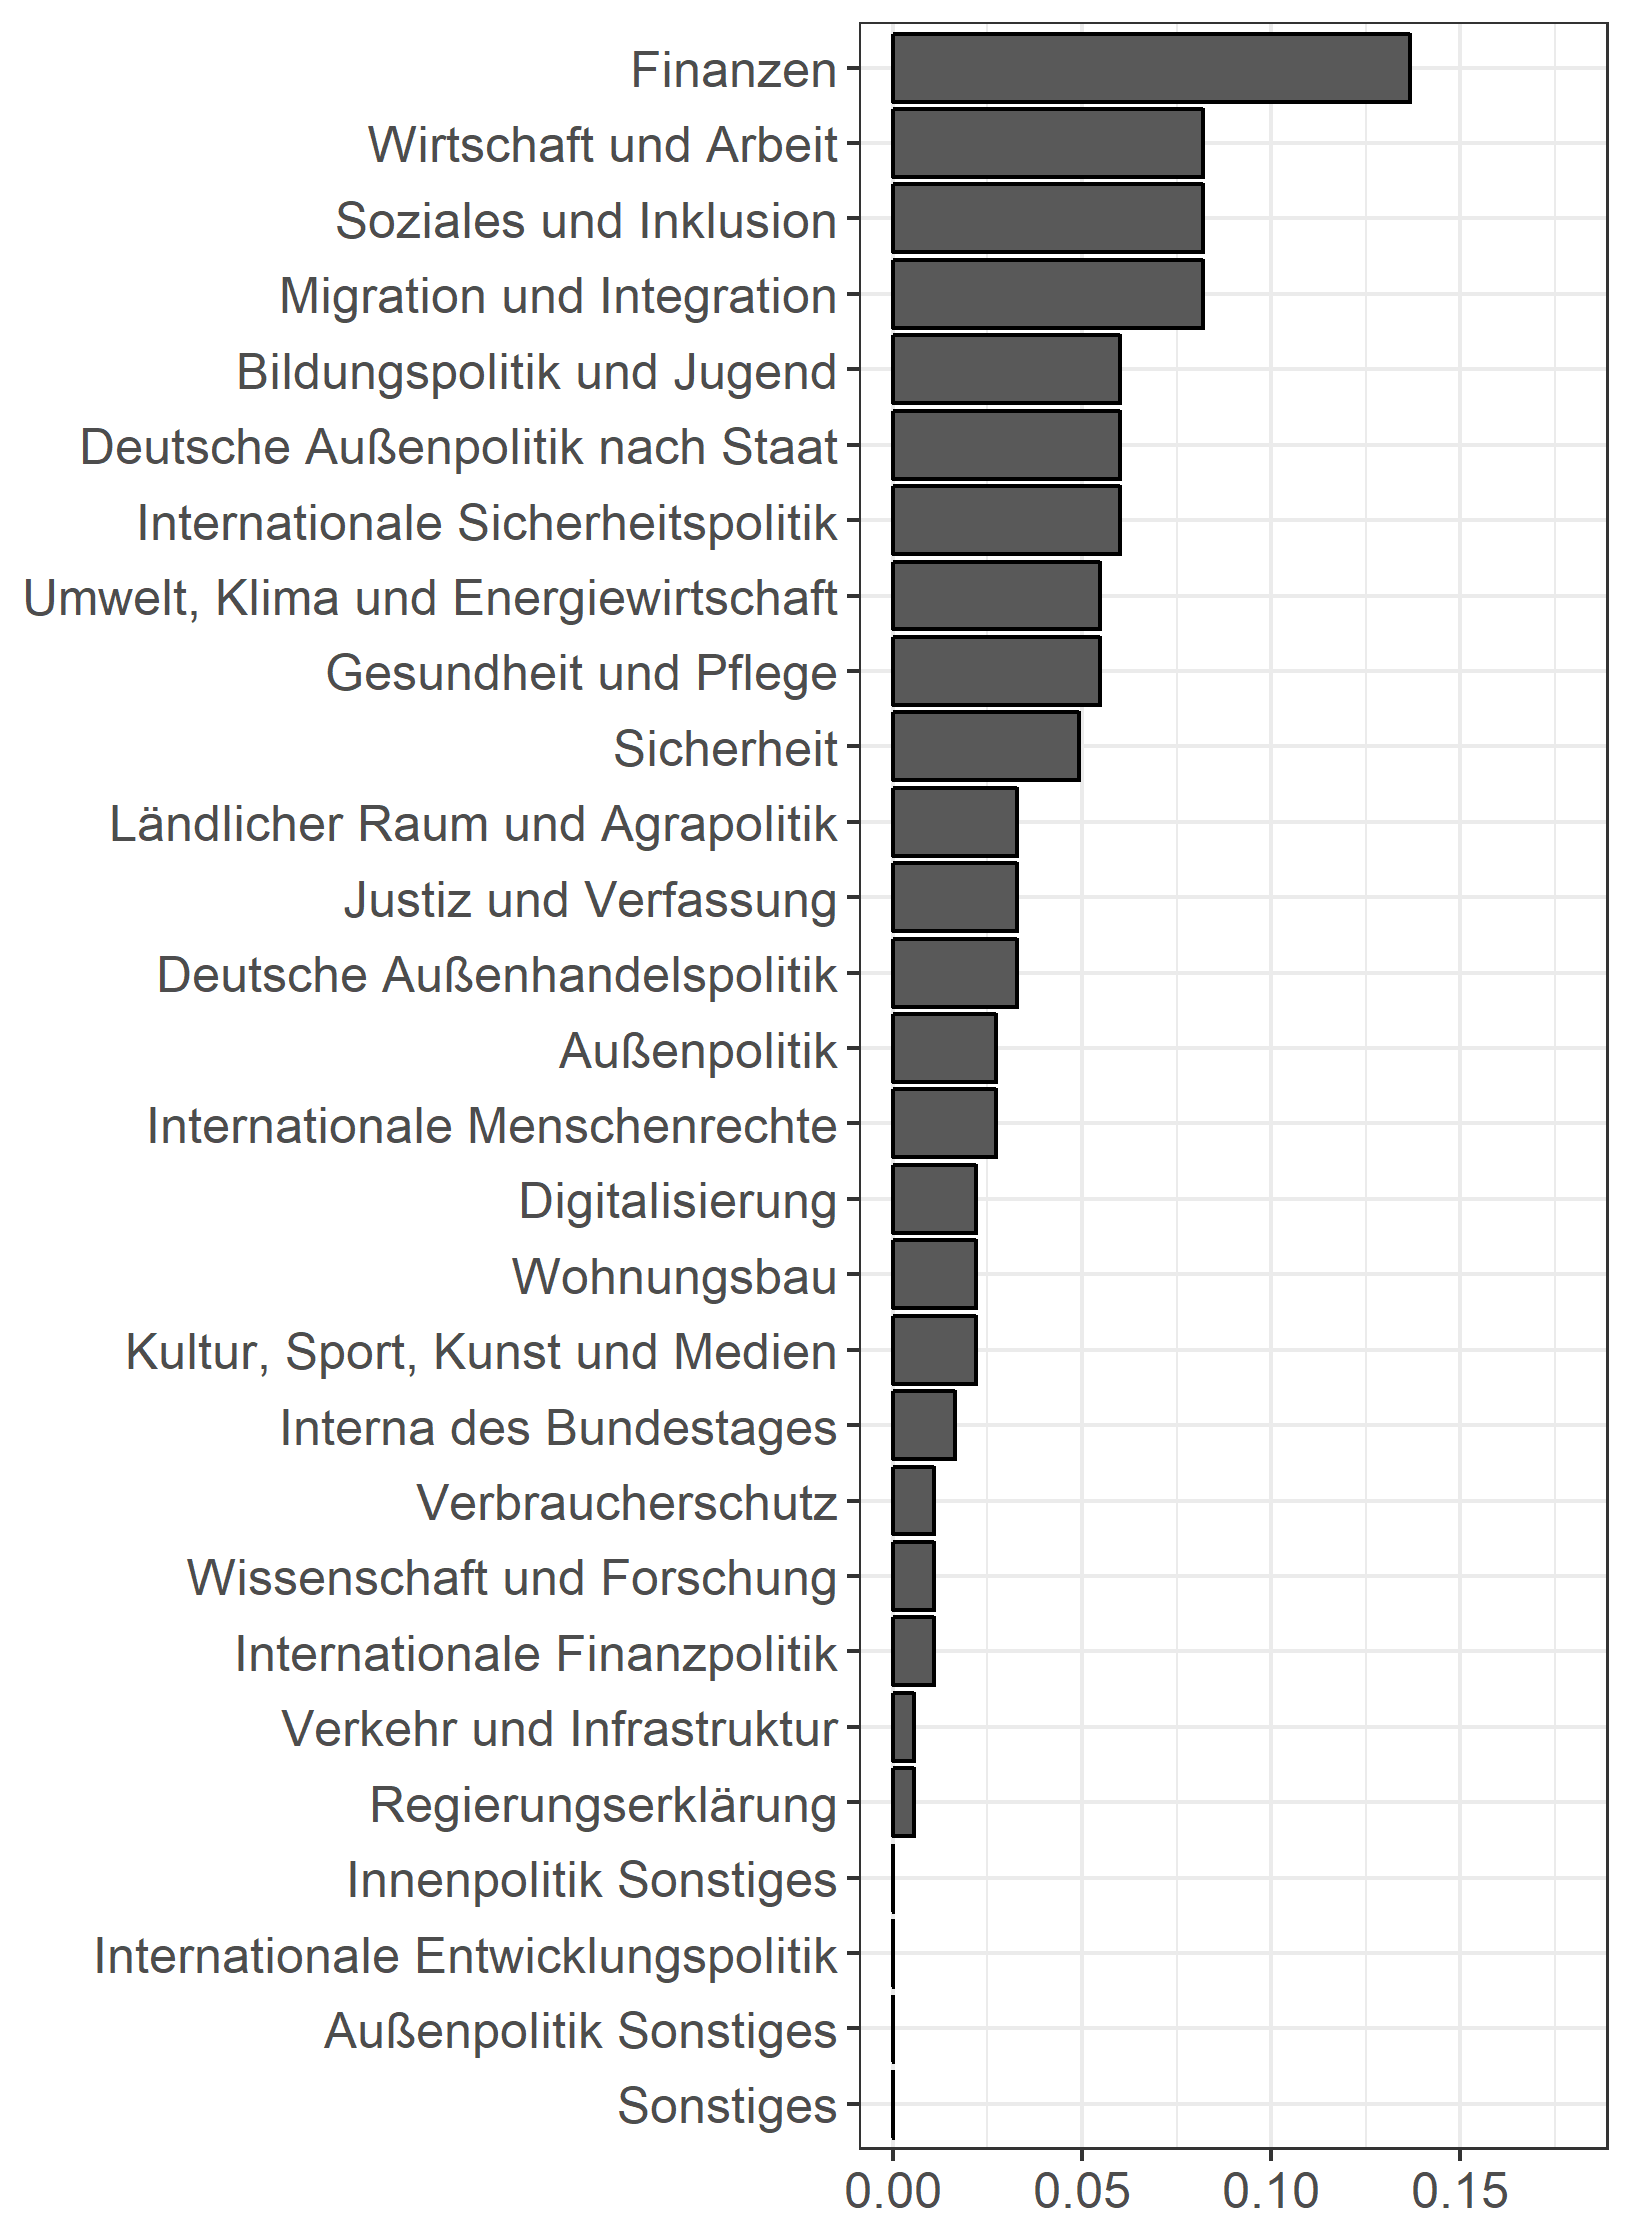
\includegraphics[width=0.29\textwidth]{Grafiken/Inhalt14.png}}
	\caption{Vergleich der Inhalte}
\end{figure}

\subsection{Inhaltliche Distanz zum TOP}

Die inhaltliche Distanz zum Tagesordnungspunkt wird durch einfaches Auszählen gemessen. Jeder Tagesordnungspunkt der Stichprobe wurde kodiert mit einem oder mehreren Inhaltsvariablen. Die Distanz ist für uns definiert durch die Häufigkeit von Redeinhalten, die vom Inhalt des Tagesordnungspunktes abweichen, geteilt durch die Anzahl aller Reden. \\
 
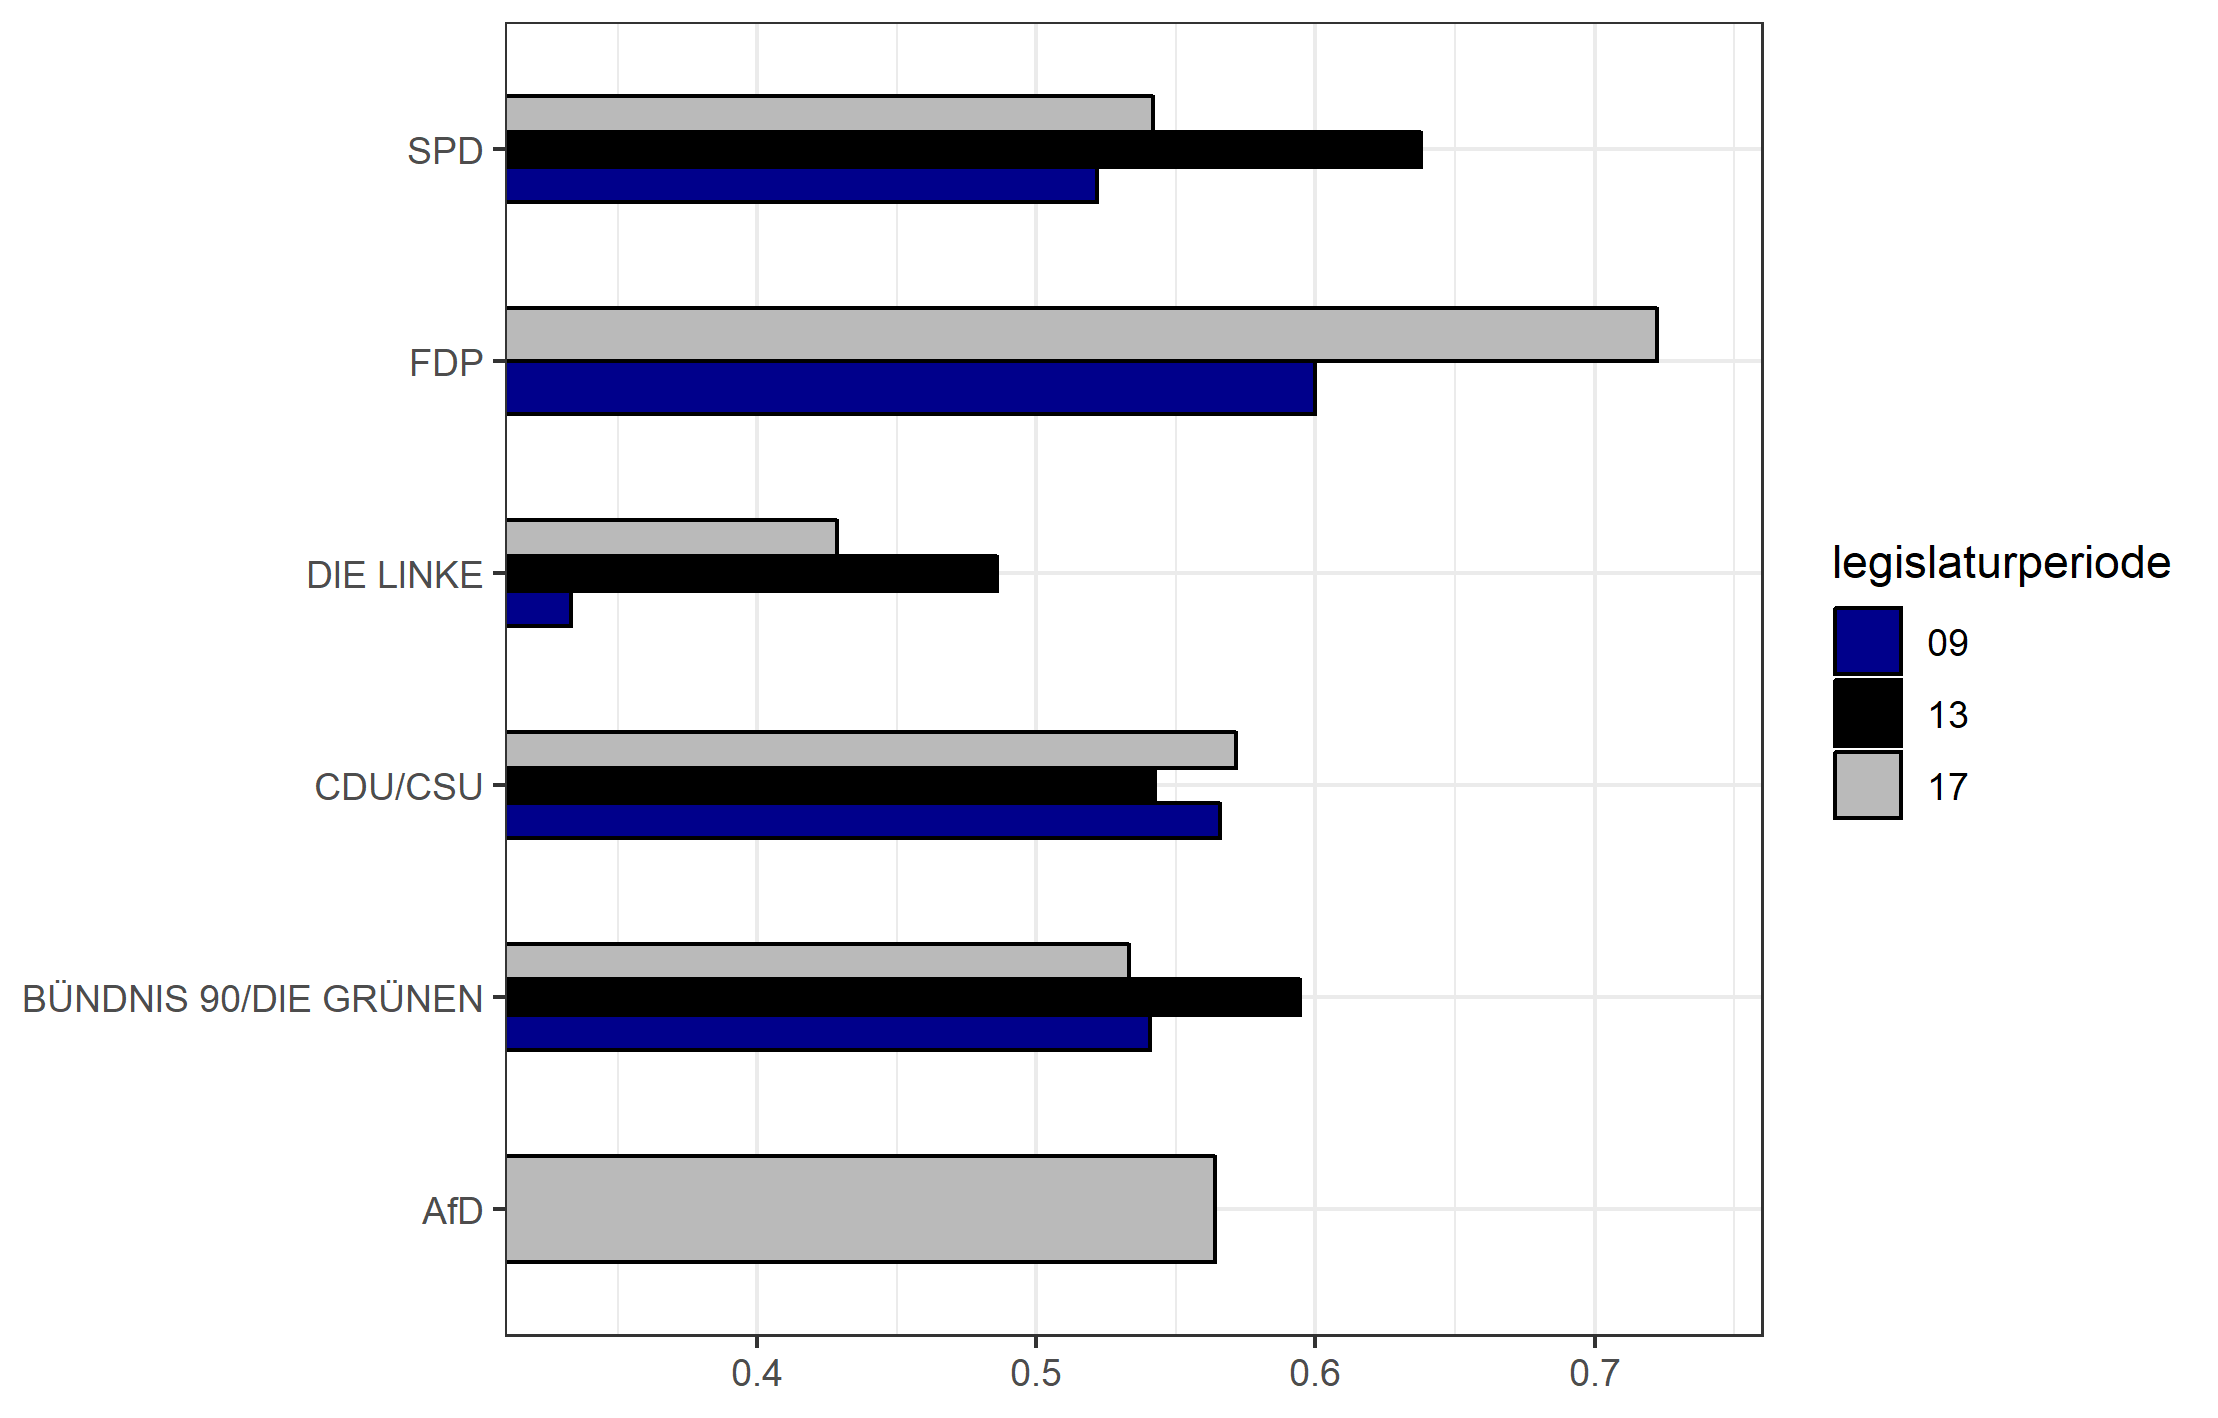
\includegraphics[width=\linewidth]{Grafiken/distop.png}\\


\subsection{Sentiment}

Die diktionär-basierte Sentimentanalyse hat keine nutzbaren Ergebnisse geliefert. Verwendet wurde das Wörterbuch der Uni- Leipzig (Quelle:), das gewichtete positive und negative Wörter enthält. \\

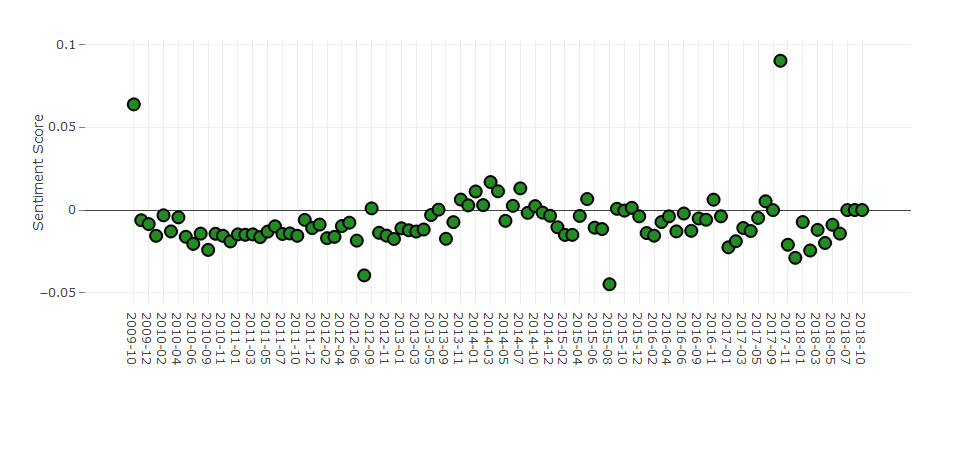
\includegraphics[width=\linewidth]{Grafiken/Sentimentscore.png}\\
\\

\subsection{Reliabilität der Stichprobe} 
\begin{table}[ht]
	\centering
	\begin{tabular}{rrrrr}
		\hline
		Variable & Mehmet und Nils & Mehmet und Vivian & Vivian und Nils & Durchschnitt \\ 
		\hline \hline
		v105 & / & 0.94 & / & / \\ 
		v300 & 0.93 & 0.75 & 1.00 & 0.83 \\ 
		v219 & / & / & 0.93 & / \\ 
		v206 & 0.93 & 0.94 & 1.00 & 0.96 \\ 
		v205 & 0.79 & 0.88 & 0.93 & 0.89 \\ 
		v204 & / & / & 1.00 & / \\ 
		v203 & 0.93 & 0.94 & 0.71 & 0.86 \\ 
		v202 & 0.79 & 0.75 & 0.93 & 0.81 \\ 
		v201 & 0.86 & 0.81 & 0.93 & 0.85 \\ 
		v119 & 0.93 & 0.94 & 0.86 & 0.91 \\ 
		v116 & 0.86 & 1.00 & 0.79 & 0.93 \\ 
		v115 & 1.00 & 1.00 & 1.00 & 1.00 \\ 
		v114 & 0.86 & 0.81 & 0.86 & 0.83 \\ 
		v113 & 0.93 & 0.81 & 0.86 & 0.83 \\ 
		v112 & 1.00 & 0.94 & 0.79 & 0.89 \\ 
		v111 & 1.00 & 0.88 & 0.79 & 0.85 \\ 
		v110 & 0.86 & 0.88 & 0.93 & 0.89 \\ 
		v109 & 0.86 & 0.88 & 1.00 & 0.92 \\ 
		v108 & 1.00 & 1.00 & 1.00 & 1.00 \\ 
		v107 & 0.79 & 0.69 & 0.86 & 0.74 \\ 
		v106 & 0.93 & 1.00 & 1.00 & 1.00 \\ 
		v104 & 0.93 & 0.94 & 1.00 & 0.96 \\ 
		v103 & 0.79 & 0.88 & 0.86 & 0.87 \\ 
		v102 & 0.79 & 0.62 & 0.71 & 0.65 \\ 
		v101 & 0.57 & 0.50 & 0.71 & 0.57 \\ 
		\hline
	\end{tabular}
\end{table}





	\section{Discussion}
	
	%===================References=====================
	\newpage
	
	\section{Bibliography}
	%\nocite{*}
	\bibliography{Quellen/Joseph}
	\newpage
	
	\section{Appendix}
	
	\listoftables
	\listoffigures
	 
	
	%===================End Document===================
\end{document}